% Options for packages loaded elsewhere
\PassOptionsToPackage{unicode}{hyperref}
\PassOptionsToPackage{hyphens}{url}
\documentclass[
]{article}
\usepackage{xcolor}
\usepackage[margin=1in]{geometry}
\usepackage{amsmath,amssymb}
\setcounter{secnumdepth}{-\maxdimen} % remove section numbering
\usepackage{iftex}
\ifPDFTeX
  \usepackage[T1]{fontenc}
  \usepackage[utf8]{inputenc}
  \usepackage{textcomp} % provide euro and other symbols
\else % if luatex or xetex
  \usepackage{unicode-math} % this also loads fontspec
  \defaultfontfeatures{Scale=MatchLowercase}
  \defaultfontfeatures[\rmfamily]{Ligatures=TeX,Scale=1}
\fi
\usepackage{lmodern}
\ifPDFTeX\else
  % xetex/luatex font selection
  \setmainfont[]{TeX Gyre Termes}
  \setmathfont[]{TeX Gyre Termes Math}
\fi
% Use upquote if available, for straight quotes in verbatim environments
\IfFileExists{upquote.sty}{\usepackage{upquote}}{}
\IfFileExists{microtype.sty}{% use microtype if available
  \usepackage[]{microtype}
  \UseMicrotypeSet[protrusion]{basicmath} % disable protrusion for tt fonts
}{}
\makeatletter
\@ifundefined{KOMAClassName}{% if non-KOMA class
  \IfFileExists{parskip.sty}{%
    \usepackage{parskip}
  }{% else
    \setlength{\parindent}{0pt}
    \setlength{\parskip}{6pt plus 2pt minus 1pt}}
}{% if KOMA class
  \KOMAoptions{parskip=half}}
\makeatother
\usepackage{longtable,booktabs,array}
\newcounter{none} % for unnumbered tables
\usepackage{calc} % for calculating minipage widths
% Correct order of tables after \paragraph or \subparagraph
\usepackage{etoolbox}
\makeatletter
\patchcmd\longtable{\par}{\if@noskipsec\mbox{}\fi\par}{}{}
\makeatother
% Allow footnotes in longtable head/foot
\IfFileExists{footnotehyper.sty}{\usepackage{footnotehyper}}{\usepackage{footnote}}
\makesavenoteenv{longtable}
\usepackage{graphicx}
\makeatletter
\newsavebox\pandoc@box
\newcommand*\pandocbounded[1]{% scales image to fit in text height/width
  \sbox\pandoc@box{#1}%
  \Gscale@div\@tempa{\textheight}{\dimexpr\ht\pandoc@box+\dp\pandoc@box\relax}%
  \Gscale@div\@tempb{\linewidth}{\wd\pandoc@box}%
  \ifdim\@tempb\p@<\@tempa\p@\let\@tempa\@tempb\fi% select the smaller of both
  \ifdim\@tempa\p@<\p@\scalebox{\@tempa}{\usebox\pandoc@box}%
  \else\usebox{\pandoc@box}%
  \fi%
}
% Set default figure placement to htbp
\def\fps@figure{htbp}
\makeatother
% definitions for citeproc citations
\NewDocumentCommand\citeproctext{}{}
\NewDocumentCommand\citeproc{mm}{%
  \begingroup\def\citeproctext{#2}\cite{#1}\endgroup}
\makeatletter
 % allow citations to break across lines
 \let\@cite@ofmt\@firstofone
 % avoid brackets around text for \cite:
 \def\@biblabel#1{}
 \def\@cite#1#2{{#1\if@tempswa , #2\fi}}
\makeatother
\newlength{\cslhangindent}
\setlength{\cslhangindent}{1.5em}
\newlength{\csllabelwidth}
\setlength{\csllabelwidth}{3em}
\newenvironment{CSLReferences}[2] % #1 hanging-indent, #2 entry-spacing
 {\begin{list}{}{%
  \setlength{\itemindent}{0pt}
  \setlength{\leftmargin}{0pt}
  \setlength{\parsep}{0pt}
  % turn on hanging indent if param 1 is 1
  \ifodd #1
   \setlength{\leftmargin}{\cslhangindent}
   \setlength{\itemindent}{-1\cslhangindent}
  \fi
  % set entry spacing
  \setlength{\itemsep}{#2\baselineskip}}}
 {\end{list}}
\usepackage{calc}
\newcommand{\CSLBlock}[1]{\hfill\break\parbox[t]{\linewidth}{\strut\ignorespaces#1\strut}}
\newcommand{\CSLLeftMargin}[1]{\parbox[t]{\csllabelwidth}{\strut#1\strut}}
\newcommand{\CSLRightInline}[1]{\parbox[t]{\linewidth - \csllabelwidth}{\strut#1\strut}}
\newcommand{\CSLIndent}[1]{\hspace{\cslhangindent}#1}
\setlength{\emergencystretch}{3em} % prevent overfull lines
\providecommand{\tightlist}{%
  \setlength{\itemsep}{0pt}\setlength{\parskip}{0pt}}
% Fix run-in paragraph style for ##### headers
\usepackage{titlesec}
\titleformat{\paragraph}[block]{\normalfont\normalsize\bfseries}{\theparagraph}{1em}{}
\titlespacing*{\paragraph}{0pt}{3.25ex plus 1ex minus .2ex}{0.5em}
\titleformat{\subparagraph}[block]{\normalfont\normalsize\bfseries}{\thesubparagraph}{1em}{}
\titlespacing*{\subparagraph}{0pt}{3.25ex plus 1ex minus .2ex}{0.5em}

% Table packages for tabularx with custom column types
\usepackage{microtype}
\frenchspacing
\usepackage{booktabs}
\usepackage{tabularx}
\usepackage{array}
\usepackage{xcolor}
\usepackage[framemethod=tikz]{mdframed}
\newcolumntype{Y}{>{\raggedright\arraybackslash}X}

% Box all Markdown blockquotes (Pandoc uses the quote environment)
% Use mdframed for stable full borders with no left/right clipping.
\mdfdefinestyle{kcorquote}{%
  linecolor=black,
  linewidth=0.4pt,
  backgroundcolor=white,
  innerleftmargin=6pt,
  innerrightmargin=6pt,
  innertopmargin=6pt,
  innerbottommargin=6pt,
  leftmargin=0pt,
  rightmargin=0pt,
  skipabove=10pt,
  skipbelow=10pt,
  topline=true,
  bottomline=true,
  leftline=true,
  rightline=true,
  roundcorner=0pt,
  splittopskip=0pt,
  splitbottomskip=0pt
}
\renewenvironment{quote}{\begin{mdframed}[style=kcorquote]}{\end{mdframed}}

% Appendix lettered numbering for figures and equations.
%
% In this repo, the manuscript uses "##" headings, which Pandoc maps to \subsection.
% There are no \section-level headings, so relying on subsection/section counters
% yields 0.x-style numbering. Instead, we define an appendix-letter counter that
% advances once per appendix (\subsection after \appendix) and resets figure/equation
% numbering within each appendix.
\usepackage{etoolbox}
\newif\ifkcorappendix
\newcounter{kcorappendix}
\pretocmd{\appendix}{%
  \kcorappendixtrue%
  \setcounter{kcorappendix}{0}%
  \renewcommand{\thefigure}{\Alph{kcorappendix}.\arabic{figure}}%
  \renewcommand{\theequation}{\Alph{kcorappendix}.\arabic{equation}}%
  \renewcommand{\thetable}{\Alph{kcorappendix}.\arabic{table}}%
}{}{}
\pretocmd{\subsection}{%
  \ifkcorappendix%
    \stepcounter{kcorappendix}%
    \setcounter{figure}{0}%
    \setcounter{equation}{0}%
    \setcounter{table}{0}%
  \fi%
}{}{}

% Disable TeX hyphenation (reviewer-friendly) and avoid PDF soft-hyphen artifacts.
% Note: this does not prevent manual hyphens, only automatic word-breaking.
\usepackage{ragged2e}
\RaggedRight
\hyphenpenalty=10000
% Allow line breaks at *explicit* hyphens that already exist in the text.
% (Keep automatic hyphenation disabled via \hyphenpenalty above.)
\exhyphenpenalty=50
\pretolerance=10000
\tolerance=2000
\emergencystretch=3em

% Suppress XeLaTeX "Missing character" warnings for Unicode math symbols.
% When math like $\theta$ appears in table cells, XeLaTeX checks if the text font
% has the Unicode math character (U+1D703 = mathematical italic theta), generating
% a warning even though the math font handles rendering correctly.
% \tracinglostchars=0 is the TeX primitive that controls this warning level:
%   0 = no warnings, 1 = warnings in log only, 2 = warnings + terminal (default)
\tracinglostchars=0

\usepackage{bookmark}
\IfFileExists{xurl.sty}{\usepackage{xurl}}{} % add URL line breaks if available
\urlstyle{same}
\hypersetup{
  hidelinks,
  pdfcreator={LaTeX via pandoc}}

\author{}
\date{}

\begin{document}

\section{KCOR: A depletion-neutralized framework for retrospective
cohort comparison under latent
frailty}\label{kcor-a-depletion-neutralized-framework-for-retrospective-cohort-comparison-under-latent-frailty}

\subsection{Manuscript metadata}\label{manuscript-metadata}

\begin{itemize}
\tightlist
\item
  \textbf{Article type}: Methods / Statistical method
\item
  \textbf{Running title}: KCOR under selection-induced cohort bias
\item
  \textbf{Author}: Steven T. Kirsch
\item
  \textbf{Affiliations}: Independent Researcher, United States
\item
  \textbf{Corresponding author}: stk@alum.mit.edu
\item
  \textbf{Word count}: 10,909 (excluding Abstract and References)
\item
  \textbf{Keywords}: selection bias; frailty model; gamma mixture model;
  frailty inversion; frailty heterogeneity; selection-induced depletion;
  non-proportional hazards; cumulative hazard; hazard normalization;
  cumulative hazards; estimands; gamma frailty; negative controls;
  observational studies; observational cohort studies
\end{itemize}

\subsection{Abstract}\label{abstract}

Selection-induced depletion under latent frailty heterogeneity can
generate non-proportional hazards and curvature in observed cumulative
hazards, biasing standard survival estimands in retrospective cohort
studies using registry and administrative data. KCOR is a
depletion-neutralized cohort comparison framework that uses a
gamma-frailty working model with a Gompertz baseline to estimate
enrollment-time frailty variance \(\theta_{0,d}\) after a prespecified
stabilization skip. The core estimator fits a seed
\((k_d,\theta_{0,d}^{(0)})\) in the nearest quiet window, reconstructs
the effective cumulative hazard over the full trajectory, aligns
multiple quiet windows through persistent wave-offset terms, and refits
\(\theta_{0,d}\) jointly across all prespecified quiet windows before
applying gamma-frailty inversion. In epidemic-wave applications, an
optional non-proportional-hazard (NPH) extension rescales wave-period
hazards before cumulative-hazard accumulation and inversion. Across
\(\theta_0\) recovery simulations, negative and positive controls, and
Cox comparison exercises, KCOR remains a diagnostic and descriptive
framework: it targets cumulative contrasts after depletion normalization
rather than counterfactual effects. This revised architecture replaces a
single-window constant-baseline fit with a more explicit identification
strategy for retrospective cohort comparisons under selection-induced
hazard curvature.

\subsection{1. Introduction}\label{introduction}

\subsubsection{1.1 Retrospective cohort comparisons under
selection}\label{retrospective-cohort-comparisons-under-selection}

Randomized controlled trials (RCTs) are the gold standard for causal
inference, but are often infeasible, underpowered for rare outcomes, or
unavailable for questions that arise after rollout. As a result,
observational cohort comparisons are widely used to estimate
intervention effects on outcomes such as all-cause mortality.

Although mortality is used throughout this paper as a motivating and
concrete example, the method applies more generally to any irreversible
event process observed in a fixed cohort, including hospitalization,
disease onset, or other terminal or absorbing states. Mortality is
emphasized here because it is objectively defined, reliably recorded in
many national datasets, and free from outcome-dependent ascertainment
biases that complicate other endpoints.

However, when intervention uptake is voluntary, prioritized, or
otherwise selective, treated and untreated cohorts are frequently
\textbf{non-exchangeable} at baseline and evolve differently over
follow-up. This problem is not limited to any single intervention class;
it arises whenever the same factors that influence treatment uptake also
influence outcome risk.

This manuscript is a methods paper. Real-world registry data are used
solely to illustrate estimator behavior, diagnostics, and failure modes
under realistic selection-induced non-proportional hazards; no policy
conclusions are drawn. KCOR does not attempt to recover counterfactual
survival curves or causal vaccine-effect estimates, and readers seeking
causal VE should not expect them here.

\subsubsection{1.2 Curvature (shape) is the hard part: non-proportional
hazards from frailty
depletion}\label{curvature-shape-is-the-hard-part-non-proportional-hazards-from-frailty-depletion}

Selection does not merely shift mortality \textbf{levels}; it can alter
mortality \textbf{curvature}---the time-evolution of cohort hazards.
Frailty heterogeneity and selection-induced depletion (depletion of
susceptibles) naturally induce curvature of the cumulative hazard even
when individual-level hazards are simple functions of time. When
selection concentrates high-frailty individuals into one cohort (or
preferentially removes them from another), the resulting cohort-level
hazard trajectories can be strongly non-proportional.

This violates core assumptions of many standard tools:

\begin{itemize}
\tightlist
\item
  \textbf{Cox PH}: assumes hazards differ by a time-invariant
  multiplicative factor (proportional hazards).
\item
  \textbf{IPTW / matching}: can balance measured covariates yet fail to
  balance unmeasured frailty and the resulting depletion dynamics.
\item
  \textbf{Age-standardization}: adjusts levels across age strata but
  does not remove cohort-specific time-evolving hazard shape.
\end{itemize}

KCOR is designed for this failure mode: \textbf{cohorts whose hazards
are not proportional because selection induces different depletion
dynamics (curvature).} In the revised estimator, curvature is
interpreted through an explicit working model: a Gompertz baseline
hazard combined with gamma-frailty depletion and an enrollment-time
frailty variance \(\theta_{0,d}\) defined at rebased time \(t=0\) after
the stabilization skip. Approximate linearity after normalization
remains a diagnostic, but no longer serves as the sole identification
anchor.

The methodological problem addressed here is general. The COVID-19
period provides a natural empirical regime characterized by strong
selection heterogeneity and non-proportional hazards, serving as a
useful illustration for the proposed framework. The \textbf{core} KCOR
estimator identifies \(\theta_{0,d}\) from prespecified quiet windows
but applies depletion normalization to the full post-enrollment
trajectory. For epidemic-wave applications, KCOR also supports an
\textbf{optional} NPH extension that adjusts wave-period hazards before
inversion; this extension is context-specific and is not part of the
universal definition of KCOR. KCOR is therefore not specific to COVID,
vaccination, or infectious disease, even though COVID-era registries
motivate one important extension module.

Two mechanisms often lumped as the `healthy vaccinee effect' (HVE) are
distinguished here:

\begin{itemize}
\item
  \textbf{Static HVE:} baseline differences in latent frailty
  distributions at cohort entry (e.g., vaccinated cohorts are healthier
  on average). In the KCOR framework, this manifests as differing
  enrollment-time frailty variance \(\theta_{0,d}\) and is the primary
  target of frailty normalization.
\item
  \textbf{Dynamic HVE:} short-horizon, time-local selection processes
  around enrollment that create transient hazard suppression immediately
  after enrollment (e.g., deferral of vaccination during acute illness,
  administrative timing, or short-term behavioral/health-seeking
  changes). Dynamic HVE is operationally addressed by prespecifying a
  skip/stabilization window (§2.7), which also defines the rebased time
  origin at which \(\theta_{0,d}\) is interpreted.
\end{itemize}

In epidemic-wave applications, an additional complication arises from
external non-proportional hazards that interact with baseline frailty.
In this manuscript, that issue is handled through an optional
epidemic-wave extension module described in Methods §2.7.1 and revisited
in Limitations §5.4.

\begin{quote}
\textbf{Box 1. Two fundamentally different strategies for cohort
comparability}

\begin{itemize}
\item
  \textbf{Traditional matching and regression approaches:} attempt to
  construct comparable cohorts by matching or adjusting
  \emph{characteristics of living individuals} at baseline or over
  follow-up, and then estimating effects via a fitted hazard model
  (e.g., Cox proportional hazards). This implicitly assumes that
  sufficiently rich covariate information can render cohorts
  exchangeable with respect to unobserved mortality risk.
\item
  \textbf{Problem under latent frailty:} even meticulous 1:1 matching on
  observed covariates can fail to equalize mortality risk trajectories.
  In such settings, cohort differences arise not from mismeasured
  covariates, but from \textbf{selection-induced depletion of
  susceptibles}, which alters hazard curvature over time.
\item
  \textbf{KCOR strategy:} rather than equating cohorts based on
  characteristics of the living, KCOR equates cohorts based on how they
  die in aggregate. It estimates cohort-specific enrollment-time
  depletion geometry through a Gompertz-plus-frailty working model
  anchored at rebased \(t=0\), aligns prespecified quiet windows through
  a structured delta-iteration estimator, removes that geometry via
  analytic inversion, and compares cohorts on the resulting
  depletion-neutralized cumulative hazard scale.
\item
  \textbf{Inferential distinction:} Cox-type methods are
  \textbf{model-based and individual-level}, conditioning on survival
  and fitting covariate effects, whereas KCOR is
  \textbf{measurement-based and cohort-level}, operating directly on
  aggregated mortality trajectories without fitting covariate models.
  The inferential target is cumulative outcome accumulation rather than
  an instantaneous hazard ratio conditional on survival.
\end{itemize}
\end{quote}

\subsubsection{1.3 Related work (brief
positioning)}\label{related-work-brief-positioning}

KCOR builds on the frailty and selection-induced depletion literature in
which unobserved heterogeneity induces deceleration of cohort-level
hazards over follow-up (a standard working model is gamma
frailty)\textsuperscript{1}. KCOR's distinct contribution is not
additional hazard flexibility, but a \textbf{diagnostics-driven
normalization} of selection-induced depletion geometry in
cumulative-hazard space prior to defining a cumulative cohort contrast.
Related approaches that address non-proportional hazards (time-varying
effects, flexible parametric hazards, additive hazards) or time-varying
confounding (MSM/IPW/g-methods) target different estimands and typically
require richer longitudinal covariates than are available in minimal
registry data\textsuperscript{2--9}. Additional discussion is provided
in the Supplementary Information (SI).

Time-varying coefficient Cox models allow hazards to change over time
but do not neutralize frailty-induced depletion because estimation
remains conditional on survival; they therefore address
non-proportionality without removing selection-induced curvature.

Marginal structural models target causal effects under exchangeability
using longitudinal covariates and weighting; KCOR instead targets
descriptive cumulative contrasts under minimal data, so the estimands,
assumptions, and failure modes differ.

Flexible parametric survival models improve baseline fit but do not
resolve depletion-induced selection bias when frailty heterogeneity is
present.

\subsubsection{1.4 Evidence from the literature: residual confounding
despite meticulous
matching}\label{evidence-from-the-literature-residual-confounding-despite-meticulous-matching}

Motivating applied studies suggest that even careful matching and
adjustment can leave substantial residual differences in non-COVID
mortality and time-varying ``healthy vaccinee effect'' signatures,
consistent with selection and depletion dynamics not captured by
measured covariates\textsuperscript{10--13}.

\subsubsection{1.5 Contribution of this
work}\label{contribution-of-this-work}

This work makes four primary contributions: (i) it formalizes
selection-induced depletion under latent frailty heterogeneity as a
source of non-proportional hazards and curvature that can bias common
survival estimands; (ii) it replaces a single-window constant-baseline
fit with a Gompertz-based delta-iteration estimator that targets
enrollment-time frailty variance \(\theta_{0,d}\) across aligned quiet
windows; (iii) it separates a universal KCOR core from an optional
epidemic-wave NPH extension module; and (iv) it validates the revised
estimator using a broader stack that includes \(\theta_0\) recovery,
control analyses, Cox mismatch demonstrations, and explicit failure
signaling.

A central implication is identifiability: in minimal-data retrospective
cohorts, interpretability depends not on a single quiet window alone but
on a coherent combination of Gompertz curvature, rebased enrollment-time
anchoring, consistency across quiet windows, and diagnostics that
indicate structured depletion geometry has been identified rather than
absorbed into residual time-varying effects.

Together, these contributions position KCOR not as a replacement for
existing survival estimands, but as a prerequisite normalization step
that addresses a source of bias arising prior to model fitting in many
retrospective cohort studies.

\subsubsection{1.6 Target estimand and scope
(non-causal)}\label{target-estimand-and-scope-non-causal}

\begin{quote}
\textbf{Box 2. Target estimand and scope (non-causal)}

\begin{itemize}
\tightlist
\item
  \textbf{Primary estimand (KCOR)}: For two fixed enrollment cohorts
  \(A\) and \(B\), it is a \textbf{neutralized marginal estimand},
  defined as \[
  \mathrm{KCOR}(t)=\tilde H_{0,A}(t)/\tilde H_{0,B}(t),
  \] where \(\tilde H_{0,d}(t)\) is cohort \(d\)'s
  \textbf{depletion-neutralized baseline cumulative hazard} obtained by
  estimating enrollment-time frailty variance \(\theta_{0,d}\) from
  prespecified quiet windows and applying the gamma-frailty inversion
  (Methods §2).
\item
  \textbf{Operational summary}: KCOR proceeds by (i) freezing cohorts
  and rebasing time after a prespecified stabilization skip, (ii)
  estimating \(\theta_{0,d}\) with a Gompertz-based delta-iteration
  procedure across prespecified quiet windows, (iii) applying
  gamma-frailty inversion to the full post-enrollment cumulative hazard
  trajectory, and (iv) comparing cohorts on that normalized cumulative
  scale. In epidemic-wave settings, an optional NPH extension may be
  applied before cumulative-hazard accumulation and inversion.
\item
  \textbf{Interpretation}: KCOR is a time-indexed \textbf{cumulative}
  contrast on the depletion-neutralized scale. Values above/below 1
  indicate greater/less cumulative event accumulation in cohort \(A\)
  than \(B\) by time \(t\) after depletion normalization. KCOR is not an
  instantaneous hazard ratio.
\item
  \textbf{What it is not}: KCOR is \textbf{not} a causal effect
  estimator (no ATE/ATT) and does not recover counterfactual outcomes
  under hypothetical interventions.
\item
  \textbf{When interpretable}: Interpretation is conditional on explicit
  assumptions (fixed cohorts; shared external hazard environment;
  adequacy of the working frailty model; identifiability of
  \(\theta_{0,d}\) from prespecified quiet windows; structured
  additivity of persistent wave offsets when the delta estimator is
  used) \textbf{and} on internal diagnostics (quiet-window fit quality;
  post-normalization linearity within quiet windows; multi-window
  consistency; parameter stability to perturbation; and, when relevant,
  plausibility of the optional NPH extension).
\item
  \textbf{If diagnostics indicate non-identifiability}: the analysis is
  treated as not identified and KCOR is not reported as a ``normalized
  contrast''.
\end{itemize}
\end{quote}

\subsubsection{1.7 Paper organization and supporting information
(SI)}\label{paper-organization-and-supporting-information-si}

The main text introduces the KCOR estimator, provides a canonical
demonstration of Cox bias under frailty-driven depletion, and presents
two primary validation examples (a negative control and a stress test).
Additional validations---including positive controls---along with
extended diagnostics, empirical registry-based nulls, and detailed
simulation specifications are provided in the Supplementary Information
(SI; Sections S2 and S4.2--S4.3; Tables
\ref{tbl:si_assumptions}--\ref{tbl:si_identifiability}).

\subsection{2. Methods}\label{methods}

Mortality is used as the primary example throughout this section because
it is objectively defined and reliably recorded in many administrative
datasets.

Table \ref{tbl:notation} defines the notation used throughout the
Methods section.

For COVID-19 vaccination analyses, intervention count corresponds to the
number of vaccine doses received; more generally, this can index any
discrete exposure level.

\subsubsection{2.1 Conceptual framework and
estimand}\label{conceptual-framework-and-estimand}

Retrospective cohort differences can arise from two qualitatively
different components:

\begin{itemize}
\tightlist
\item
  \textbf{Level differences}: cohort hazards differ by an approximately
  time-stable multiplicative factor (or, equivalently, cumulative
  hazards have different slopes but similar shape).
\item
  \textbf{Depletion (curvature) differences}: cohort hazards evolve
  differently over time because cohorts differ in latent heterogeneity
  and are \textbf{selectively depleted} at different rates.
\end{itemize}

This framework targets the second failure mode. Under latent frailty
heterogeneity, high-risk individuals die earlier, so the surviving risk
set becomes progressively ``healthier.'' This induces \textbf{downward
curvature} (deceleration) in cohort hazards and corresponding concavity
in cumulative-hazard space, even when individual-level hazards are
simple and even under a true null treatment effect. When selection
concentrates frailty heterogeneity differently across cohorts, the
resulting curvature differences produce strong non-proportional hazards
and can drive misleading contrasts for estimands that condition on the
evolving risk set.

KCOR does not assert a causal interpretation of the resulting contrast;
rather, it isolates residual differences that cannot be attributed to
frailty-driven selection, thereby identifying regimes that demand
substantive explanation beyond selection artifacts. KCOR does not claim
to distinguish depletion-induced heterogeneity from constant
proportional hazard shifts within a quiet window; rather, it conditions
interpretation on the working frailty model and diagnostic adequacy.

The strategy is therefore:

\begin{enumerate}
\def\labelenumi{\arabic{enumi}.}
\tightlist
\item
  \textbf{Estimate the cohort-specific depletion geometry} (via
  curvature) during prespecified epidemiologically quiet periods.
\item
  \textbf{Map observed cumulative hazards into a depletion-neutralized
  space} by inverting that geometry.
\item
  \textbf{Compare cohorts only after normalization} using a prespecified
  post-adjustment estimand; ratios of depletion-neutralized cumulative
  hazards (KCOR) are used here.
\end{enumerate}

KCOR deliberately targets cumulative mortality contrasts rather than
instantaneous hazard ratios. This choice is intentional: cumulative
outcome accumulation is invariant to transient hazard-ratio oscillations
induced purely by depletion geometry. It is therefore not intended as a
replacement for Cox proportional hazards models or flexible parametric
survival models that estimate time-varying hazard effects. Instead, KCOR
provides a geometry-based normalization of cumulative risk in settings
where selection-induced depletion distorts marginal comparisons.

All analyses are performed using discrete weekly time bins;
continuous-time notation is used solely for expositional convenience.
See Table \ref{tbl:notation} for the full symbol list.

\textbf{Notation preview.}\\
Throughout this paper, \(t\) denotes event time since cohort enrollment
and \(d\) indexes cohorts. For frailty identification, time is rebased
after the stabilization skip so that \(t_{\mathrm{rebased}}=0\) at the
first accumulating interval. Let \(H_{\mathrm{obs},d}(t)\) denote the
observed cohort-level cumulative hazard, computed from fixed risk sets
after the required preprocessing steps, and let \(\tilde H_{0,d}(t)\)
denote the corresponding \emph{depletion-neutralized baseline cumulative
hazard} obtained after frailty normalization. Individual hazards are
modeled using a latent multiplicative frailty term \(z\), with
cohort-specific enrollment-time variance \(\theta_{0,d}\), which governs
the strength of selection-induced depletion and resulting curvature in
observed cumulative hazards. Full notation is summarized in Table
\ref{tbl:notation}.

\paragraph{2.1.1 Target estimand}\label{target-estimand}

Scope and interpretation are summarized in Box 2 (§1.6); the formal
definition used throughout is provided here.

Let \(\tilde H_{0,d}(t)\) denote the \textbf{depletion-neutralized
baseline cumulative hazard} for cohort \(d\) at event time \(t\) since
enrollment (Table \ref{tbl:notation}). For two cohorts \(A\) and \(B\),
KCOR is defined as

\begin{equation}\protect\phantomsection\label{eq:kcor-estimand}{
\mathrm{KCOR}(t) = \frac{\tilde H_{0,A}(t)}{\tilde H_{0,B}(t)}.
}\end{equation}

For visualization, an \textbf{anchored KCOR} is sometimes reported to
show post-reference divergence: \[
\mathrm{KCOR}(t; t_0) = \mathrm{KCOR}(t)/\mathrm{KCOR}(t_0),
\] with prespecified \(t_0\) (e.g., 4 weeks). Anchoring is used only
when explicitly stated to remove pre-existing level differences and
emphasize post-reference divergence.

\paragraph{2.1.2 Identification versus
diagnostics}\label{identification-versus-diagnostics}

Scope and interpretation are summarized in Box 2 (§1.6).

Interpretability of a KCOR trajectory is assessed via prespecified
diagnostics (Supplementary Information §S2; Tables
\ref{tbl:si_assumptions}--\ref{tbl:si_identifiability}). When
diagnostics indicate non-identifiability, the analysis is treated as not
identified and results are not reported. Checks include:

\begin{itemize}
\tightlist
\item
  stability of \((\hat{k}_d,\hat{\theta}_{0,d})\) and the aligned
  quiet-window geometry under small perturbations,
\item
  approximate linearity of \(\tilde H_{0,d}(t)\) within the quiet
  window,
\item
  absence of systematic residual structure in hazard space.
\end{itemize}

Diagnostics corresponding to each assumption are summarized in
Supplementary Information §S2 (Tables
\ref{tbl:si_assumptions}--\ref{tbl:si_identifiability}).

\paragraph{2.1.3 KCOR assumptions and
diagnostics}\label{kcor-assumptions-and-diagnostics}

These assumptions define when KCOR normalization is interpretable.

The KCOR framework relies on the following assumptions, which are framed
diagnostically:

\begin{enumerate}
\def\labelenumi{\arabic{enumi}.}
\item
  \textbf{Fixed cohort enrollment.} Cohorts are defined at a common
  enrollment time and followed forward without dynamic entry or
  rebalancing.
\item
  \textbf{Multiplicative latent frailty.} Individual hazards are assumed
  to be multiplicatively composed of a baseline hazard and an unobserved
  frailty term, with cohort-specific frailty distributions.
\item
  \textbf{Quiet-window stability.} A prespecified epidemiologically
  quiet period exists during which external shocks to the baseline
  hazard are minimal, allowing depletion geometry to be estimated from
  observed cumulative hazards. Residual baseline drift can be absorbed
  into the frailty parameter if quiet-window conditions are violated;
  empirical robustness of fitted frailty parameters to quiet-window
  placement (12-month windows shifted monthly) is demonstrated in
  Supplementary Figure \ref{fig:si_quiet_window_theta_scan} using Czech
  registry data. Epidemic-wave periods with sharp hazard shocks fall
  outside this assumption and are excluded from normalization by design.
\item
  \textbf{Independence across strata.} Cohorts or strata are analyzed
  independently, without interference, spillover, or cross-cohort
  coupling.
\item
  \textbf{Sufficient event-time resolution.} Event timing is observed at
  a temporal resolution adequate to estimate cumulative hazards over the
  quiet window.
\end{enumerate}

If no candidate quiet window satisfies diagnostic criteria, KCOR is not
interpretable and analysis should terminate without reporting contrasts.
Multiple disjoint quiet windows may be pooled provided fitted depletion
parameters are stable and diagnostics are consistent across windows.
Quiet-window validity diagnostics are summarized in Supplementary
Information §S2 (Tables
\ref{tbl:si_assumptions}--\ref{tbl:si_identifiability}).

These assumptions are evaluated empirically using post-normalization
diagnostics. Violations are expected to manifest as residual curvature,
drift, or instability in adjusted cumulative hazard trajectories.

\subsubsection{2.2 Cohort construction}\label{cohort-construction}

KCOR is defined for \textbf{fixed cohorts at enrollment}. Required
inputs are minimal: enrollment date(s), event date, and optionally birth
date (or year-of-birth) for age stratification. Analyses proceed in
discrete event time \(t\) (e.g., weeks) measured since cohort
enrollment.

Cohorts are assigned by intervention state at the start of the
enrollment interval. In the primary estimand:

\begin{itemize}
\tightlist
\item
  \textbf{No post-enrollment switching} is allowed (individuals remain
  in their enrollment cohort),
\item
  \textbf{No censoring} is applied (other than administrative end of
  follow-up),
\item
  analyses are performed on the resulting fixed risk sets.
\end{itemize}

Censoring or reclassification due to cohort transitions (e.g., moving
between exposure groups over time) is not permitted, because such
transitions alter the frailty composition of the cohort in a
time-dependent manner. Allowing transitions would introduce additional,
endogenous selection that changes cohort mortality trajectories in
unpredictable ways, confounding depletion effects that KCOR is designed
to normalize.

This fixed-cohort design is intentional. It avoids immortal-time
artifacts and prevents outcome-driven switching rules from creating
time-dependent selection that is difficult to diagnose under minimal
covariate availability. Extensions that allow switching or censoring are
treated as sensitivity analyses (§5.2) because they change the estimand
and introduce additional identification requirements.

Conceptual requirements of the KCOR framework are distinguished from
operational defaults, which are reported separately for reproducibility
(Supplementary Section S4).

Throughout this manuscript the failure event is \textbf{all-cause
mortality}. KCOR therefore targets cumulative mortality hazards and is
not framed as a cause-specific competing-risks analysis.

\subsubsection{2.3 Hazard estimation and cumulative hazards in discrete
time}\label{hazard-estimation-and-cumulative-hazards-in-discrete-time}

For each cohort \(d\), let \(N_d(0)\) denote the number of individuals
at enrollment. Let \(d_d(t)\) denote deaths occurring during interval
\(t\), and let \[
D_d(t) = \sum_{s \le t} d_d(s)
\] denote cumulative deaths up to the end of interval \(t\).

Define the risk set size at the start of interval \(t\) as \[
N_d(t) = N_d(0) - \sum_{s < t} d_d(s) = N_d(0) - D_d(t-1).
\] In the primary estimand, individuals do not switch cohorts after
enrollment and there is no loss to follow-up; therefore \(N_d(t)\) is
the risk set used to define all discrete-time hazards and cumulative
hazards in this manuscript.

Define the interval mortality ratio \[
\mathrm{MR}_{d,t} = \frac{d_d(t)}{N_d(t)}.
\]

The discrete-time cohort hazard is computed as

\begin{equation}\protect\phantomsection\label{eq:hazard-discrete}{
h_{\mathrm{obs},d}(t) = -\ln\!\left(1 - \mathrm{MR}_{d,t}\right) = -\ln\!\left(1 - \frac{d_d(t)}{N_d(t)}\right).
}\end{equation}

This transform is standard: it maps an interval event probability into a
continuous-time equivalent hazard under a piecewise-constant hazard
assumption. For rare events,
\(h_{\mathrm{obs},d}(t) \approx \mathrm{MR}_{d,t} = d_d(t)/N_d(t)\), but
the log form remains accurate and stable when weekly risks are not
negligible. The exact transform
\(h_{\mathrm{obs},d}(t) = -\log(1 - \mathrm{MR}_{d,t})\) is used
throughout; the rare-event approximation is provided for intuition only.
This discrete-time hazard transform under a piecewise-constant hazard
assumption is standard; see, e.g., Kalbfleisch and Prentice (\emph{The
Statistical Analysis of Failure Time Data})\textsuperscript{14}.

\emph{All hazard and cumulative-hazard quantities used in KCOR are
discrete-time integrated hazard estimators derived from fixed-cohort
risk sets; likelihood-based or partial-likelihood formulations are not
used for estimation or for the subsequent frailty-based normalization.}

Observed cumulative hazards are accumulated over event time after
preprocessing (§2.7), where preprocessing always includes the
stabilization skip and may additionally include the optional
epidemic-wave NPH extension:

\begin{equation}\protect\phantomsection\label{eq:cumhazard-observed}{
H_{\mathrm{obs},d}(t) = \sum_{s \le t} h_d^{\mathrm{adj}}(s),
\qquad \Delta t = 1.
}\end{equation}

Discrete binning accommodates tied events and aggregated registry
releases. Bin width is chosen based on diagnostic stability (e.g.,
smoothness and sufficient counts per bin) rather than temporal
resolution alone.

In addition to the primary implementation above,
\(\hat H_{\mathrm{obs},d}(t)\) was computed using the Nelson--Aalen
estimator \(\sum_{s \le t} d_d(s)/N_d(s)\) as a sensitivity check;
results were unchanged.

\subsubsection{2.4 Selection model: gamma frailty and depletion
normalization}\label{selection-model-gamma-frailty-and-depletion-normalization}

\paragraph{2.4.1 Individual hazards with multiplicative
frailty}\label{individual-hazards-with-multiplicative-frailty}

Let \(z_{i,d}\) denote an individual-specific latent frailty term with
mean \(1\) and variance \(\theta_{0,d}\), defined at rebased time
\(t_{\mathrm{rebased}}=0\) after the stabilization skip. Let
\(\tilde h_{0,d}(t)\) denote the depletion-neutralized baseline hazard
for cohort \(d\). Individual hazards are modeled as

\begin{equation}\protect\phantomsection\label{eq:individual-hazard-frailty}{
h_{i,d}(t) = z_{i,d}\,\tilde h_{0,d}(t),
\qquad
z_{i,d} \sim \mathrm{Gamma}(\mathrm{mean}=1,\ \mathrm{var}=\theta_{0,d}).
}\end{equation}

Here \(\theta_{0,d}\) is an \textbf{enrollment-time} parameter: it
characterizes the cohort's frailty heterogeneity at the start of the
accumulating follow-up, not the time-varying variance of the surviving
population after depletion has acted. Larger \(\theta_{0,d}\) produces
stronger early depletion of high-frailty individuals and therefore
stronger cohort-level hazard deceleration.

Gamma frailty is used because it yields a closed-form link between
observed and baseline cumulative hazards via the Laplace
transform\textsuperscript{1}. In KCOR, gamma frailty is a
\textbf{working geometric model} for depletion normalization, not a
claim of biological truth. Adequacy is evaluated empirically through fit
quality, multi-window consistency, and post-normalization diagnostics.

\paragraph{2.4.2 Gamma-frailty identity and
inversion}\label{gamma-frailty-identity-and-inversion}

Let

\begin{equation}\protect\phantomsection\label{eq:baseline-cumhazard}{
\tilde H_{0,d}(t) = \int_0^t \tilde h_{0,d}(s)\,ds
}\end{equation}

denote the depletion-neutralized baseline cumulative hazard. Under the
gamma-frailty working model, the observed cohort-level cumulative hazard
satisfies

\begin{equation}\protect\phantomsection\label{eq:gamma-frailty-identity}{
H_{\mathrm{obs},d}(t) = \frac{1}{\theta_{0,d}}\,\log\!\left(1 + \theta_{0,d} \tilde H_{0,d}(t)\right),
}\end{equation}

and the corresponding inversion is

\begin{equation}\protect\phantomsection\label{eq:gamma-frailty-inversion}{
\tilde H_{0,d}(t) = \frac{\exp\!\left(\theta_{0,d} H_{\mathrm{obs},d}(t)\right) - 1}{\theta_{0,d}}.
}\end{equation}

This inversion is the \textbf{normalization operator}: given an estimate
\(\hat{\theta}_{0,d}\), it maps the observed cumulative hazard
\(H_{\mathrm{obs},d}(t)\) into a depletion-neutralized cumulative hazard
scale. We use a tilde (e.g., \(\tilde H_{0,d}(t)\)) to denote
depletion-neutralized baseline quantities obtained after frailty
normalization; observed cohort-aggregated quantities are written without
a tilde (e.g., \(H_{\mathrm{obs},d}(t)\)).

\paragraph{2.4.3 Gompertz baseline and enrollment-time
interpretation}\label{gompertz-baseline-and-enrollment-time-interpretation}

To identify \(\theta_{0,d}\), the revised KCOR estimator uses a Gompertz
baseline hazard over rebased event time:

\begin{equation}\protect\phantomsection\label{eq:baseline-shape-default}{
\tilde h_{0,d}(t_{\mathrm{rebased}})=k_d e^{\gamma t_{\mathrm{rebased}}},
\qquad
H_{\mathrm{gom},d}(t_{\mathrm{rebased}})=\frac{k_d}{\gamma}\!\left(e^{\gamma t_{\mathrm{rebased}}}-1\right).
}\end{equation}

Here \(\gamma\) is a fixed Gompertz slope and \(k_d\) is a
cohort-specific scale parameter. This choice imposes more structure than
the earlier constant-baseline specification, but it aligns the estimator
with the biological age-slope assumption used in the v7.5 implementation
and makes the parameter of interest explicit: \(\theta_{0,d}\) is the
frailty variance at rebased \(t=0\), not a late-window summary of an
already depleted cohort.

\paragraph{2.4.4 Quiet-window validity and
identifiability}\label{quiet-window-validity-and-identifiability}

Frailty parameters are identified using only bins whose corresponding
calendar weeks lie inside prespecified quiet windows (defined in
ISO-week space). These windows are chosen to avoid sharp external shocks
that would confound depletion-geometry identification. In the revised
estimator, however, no single quiet window is assumed sufficient on its
own. Identification depends on:

\begin{enumerate}
\def\labelenumi{\arabic{enumi}.}
\tightlist
\item
  adequate Gompertz-plus-frailty fit within quiet windows,
\item
  consistency of \(\hat{\theta}_{0,d}\) across aligned quiet windows
  after structured offset correction,
\item
  stability to small boundary perturbations, and
\item
  plausible reconstruction of persistent wave offsets when the
  delta-iteration path is used.
\end{enumerate}

If these conditions fail, diagnostics indicate non-identifiability and
the analysis is treated as not identified rather than reported as a
stable normalized contrast. Full operational diagnostics are summarized
in Supplementary Information §S2.

\subsubsection{\texorpdfstring{2.5 Estimating \(\theta_{0,d}\) by delta
iteration}{2.5 Estimating \textbackslash theta\_\{0,d\} by delta iteration}}\label{estimating-theta_0d-by-delta-iteration}

KCOR estimates \((\hat{k}_d,\hat{\theta}_{0,d})\) independently for each
cohort \(d\) using a structured four-step procedure. Throughout this
section, let \(h_d^{\mathrm{adj}}(t)\) denote the preprocessed hazard
used for accumulation and fitting: in the core estimator
\(h_d^{\mathrm{adj}}(t)=h_d^{\mathrm{eff}}(t)\), while in epidemic-wave
applications it may include the optional NPH adjustment defined in
§2.7.1.

Let \(W_{0,d}\) denote the nearest quiet window after enrollment and let
\(\bigcup_j W_{j,d}\) denote the union of all prespecified quiet windows
for cohort \(d\), both evaluated on rebased time with
\(t_{\mathrm{rebased}} \ge 0\).

\textbf{Step 1: joint seed fit in the nearest quiet window.}\\
Estimate \((k_d,\theta_{0,d}^{(0)})\) from the nearest quiet window by
nonlinear least squares in hazard space:

\begin{equation}\protect\phantomsection\label{eq:nls-objective}{
(\hat{k}_d,\hat{\theta}_{0,d}^{(0)})
=
\arg\min_{k_d>0,\ \theta_{0,d}\ge0}
\sum_{t \in W_{0,d}}
\left[
h_d^{\mathrm{adj}}(t)-
\frac{k_d e^{\gamma t_{\mathrm{rebased}}}}{1+\theta_{0,d} H_{\mathrm{gom},d}(t_{\mathrm{rebased}})}
\right]^2 .
}\end{equation}

This seed fit anchors the Gompertz scale parameter \(\hat{k}_d\) close
to enrollment and avoids identifying \(\theta_{0,d}\) from a late,
already depleted population.

\textbf{Step 2: reconstruct the effective cumulative hazard over the
full trajectory.}\\
Given the current iterate \(\hat{\theta}_{0,d}^{(m)}\), reconstruct the
effective individual-level hazard and cumulative hazard over
\textbf{all} observed weeks:

\[
h_{0,d}^{\mathrm{eff}}(t)=h_d^{\mathrm{adj}}(t)\left(1+\hat{\theta}_{0,d}^{(m)}H_{0,d}^{\mathrm{eff}}(t)\right),
\qquad
H_{0,d}^{\mathrm{eff}}(t+1)=H_{0,d}^{\mathrm{eff}}(t)+h_{0,d}^{\mathrm{eff}}(t),
\]

starting from \(H_{0,d}^{\mathrm{eff}}(0)=0\).

\textbf{Step 3: compute persistent wave offsets.}\\
For each prespecified wave end time \(t_i\), compute the incremental
offset

\[
\delta_{i,d}
=
\left[H_{0,d}^{\mathrm{eff}}(t_i)-H_{\mathrm{gom},d}(t_i)\right]-\sum_{j<i}\delta_{j,d},
\qquad
\Delta_d(t)=\sum_{i:\,t_i\le t}\delta_{i,d}.
\]

This step encodes the structural assumption that wave effects are
additive in cumulative-hazard space and persist after the wave ends.
Implausible offset behavior is treated diagnostically; detailed fallback
rules are provided in the Supplementary Information.

\textbf{Step 4: pooled refit across all quiet windows.}\\
Holding \(\hat{k}_d\) fixed, refit \(\theta_{0,d}\) across the union of
all quiet windows:

\[
\hat{\theta}_{0,d}
=
\arg\min_{\theta_{0,d}\ge0}
\sum_{t \in \bigcup_j W_{j,d}}
\left[
h_d^{\mathrm{adj}}(t)-
\frac{\hat{k}_d e^{\gamma t_{\mathrm{rebased}}}}{1+\theta_{0,d}\left(H_{\mathrm{gom},d}(t_{\mathrm{rebased}})+\Delta_d(t)\right)}
\right]^2 .
\]

The reconstruction and pooled refit are iterated to convergence, which
in the reference implementation typically occurs within a small number
of iterations. When curvature is weak, the delta structure is
inapplicable, or events are too sparse, the estimator may collapse
toward the \(\theta_{0,d}\to0\) limit; this is interpreted as weak
identifiability rather than as evidence for or against any particular
cohort.

All analyses use a prespecified reference implementation with fixed
operational defaults; full derivations, convergence notes, and edge-case
rules are provided in Supplementary Section S4.

\subsubsection{2.6 Normalization (depletion-neutralized cumulative
hazards)}\label{normalization-depletion-neutralized-cumulative-hazards}

After fitting, KCOR computes the depletion-neutralized baseline
cumulative hazard for each cohort \(d\) by applying the inversion to the
full post-enrollment trajectory:

\begin{equation}\protect\phantomsection\label{eq:normalized-cumhazard}{
\tilde H_{0,d}(t) = \frac{\exp\!\left(\hat{\theta}_{0,d}\,H_{\mathrm{obs},d}(t)\right)-1}{\hat{\theta}_{0,d}}.
}\end{equation}

This normalization maps each cohort into a depletion-neutralized
baseline-hazard space in which the contribution of gamma frailty
parameters \((\hat{\theta}_{0,d}, \hat{k}_d)\) to hazard curvature has
been factored out. The inversion is always applied to the full observed
cumulative hazard trajectory after preprocessing. In the core estimator
that preprocessing is the stabilization skip; in epidemic-wave
applications it may also include the optional NPH extension. This
normalization defines a common comparison scale in cumulative-hazard
space; it is not equivalent to Cox partial-likelihood baseline
anchoring, but serves an analogous geometric role for cumulative
contrasts. The core identities used in KCOR are given in Equations
(\ref{eq:hazard-discrete}), (\ref{eq:nls-objective}),
(\ref{eq:normalized-cumhazard}), and (\ref{eq:kcor-estimand}).
Normalization defines a common comparison scale; the scientific estimand
is then computed on that scale (Box 2).

\paragraph{2.6.1 Computational
considerations}\label{computational-considerations}

KCOR operates on aggregated event counts in discrete time and
cumulative-hazard space. Computational complexity scales linearly with
the number of time bins and strata rather than the number of
individuals, making the method feasible for very large population
registries. In practice, KCOR analyses on national-scale datasets
(millions of individuals) are memory-bound rather than CPU-bound and can
be implemented efficiently using standard vectorized numerical
libraries. No iterative optimization over individual-level records is
required. \textbf{Numerical stability at vanishing frailty variance.}\\
When the fitted frailty variance satisfies
\(\hat\theta_{0,d} < \varepsilon\) (with \(\varepsilon\) set to a small
numerical tolerance, e.g., \(10^{-8}\)), the gamma-frailty inversion in
Eq. ((\ref{eq:normalized-cumhazard})) is evaluated in the
\(\theta_0 \to 0\) limit, yielding \[
\tilde H_{0,d}(t)=H_{\mathrm{obs},d}(t),
\] which corresponds to the standard Nelson--Aalen cumulative hazard.
This avoids numerical instability from evaluating
\((\exp(\theta_0 H)-1)/\theta_0\) near machine precision and reflects
the fact that near-zero fitted \(\theta_0\) indicates negligible
detectable depletion curvature.

\paragraph{2.6.2 Internal diagnostics and `self-check'
behavior}\label{internal-diagnostics-and-self-check-behavior}

KCOR includes internal diagnostics intended to make model stress visible
rather than hidden.

\begin{enumerate}
\def\labelenumi{\arabic{enumi}.}
\item
  \textbf{Post-normalization linearity in quiet periods.} Within
  prespecified quiet windows (see §2.4.4), the depletion-neutralized
  cumulative hazard should be approximately linear in rebased event time
  after inversion. Systematic residual curvature indicates contaminated
  windows, misspecified depletion geometry, or failure of the offset
  structure.
\item
  \textbf{Fit residual structure in hazard space.} Define residuals over
  the pooled fit set:
\end{enumerate}

\begin{equation}\protect\phantomsection\label{eq:si_residuals}{
r_{d}(t)=h_d^{\mathrm{adj}}(t)-\frac{\hat{k}_d e^{\gamma t_{\mathrm{rebased}}}}{1+\hat{\theta}_{0,d}\left(H_{\mathrm{gom},d}(t_{\mathrm{rebased}})+\Delta_d(t)\right)}.
}\end{equation}

KCOR expects residuals to be small and not systematically
time-structured within or across quiet windows. Strongly patterned
residuals indicate that the curvature attributed to depletion is instead
being driven by unmodeled time-varying hazards.

\begin{enumerate}
\def\labelenumi{\arabic{enumi}.}
\setcounter{enumi}{2}
\item
  \textbf{Multi-window stability.} Under valid quiet-window selection,
  the reconstructed offsets and fitted parameters should be stable to
  small perturbations of quiet-window boundaries and to omission of
  individual quiet windows. Large changes under minor perturbations
  signal that the fitted geometry is being driven by transient dynamics
  rather than by stable depletion structure.
\item
  \textbf{Weak identifiability manifests through boundary behavior.}
  Near-zero \(\hat{\theta}_{0,d}\), unstable \(\Delta_d(t)\), or failure
  of the offset reconstruction all indicate that \(\theta_0\) is weakly
  identified. In such cases, KCOR should be interpreted primarily as a
  diagnostic rather than as a strong normalization.
\end{enumerate}

These diagnostics are reported alongside \(\mathrm{KCOR}(t)\) curves.
The goal is not to assert that a single parametric form is always
correct, but to ensure that when the form is incorrect or the window is
contaminated, the method signals this explicitly rather than silently
producing a misleading normalized estimate. When diagnostics indicate
non-identifiability, the depletion-based normalization is inappropriate
and KCOR should not be interpreted.

\subsubsection{2.7 Stabilization (early
weeks)}\label{stabilization-early-weeks}

In many applications, the first few post-enrollment intervals can be
unstable due to immediate post-enrollment artifacts (e.g., rapid
deferral, short-term sorting, administrative effects). KCOR supports a
prespecified stabilization rule by excluding early weeks from
accumulation and from quiet-window fitting. The skip-weeks parameter is
prespecified and evaluated via sensitivity analysis to exclude early
enrollment instability rather than to tune estimates.

In discrete time, define an effective hazard for accumulation:

\begin{equation}\protect\phantomsection\label{eq:effective-hazard-skip}{
h_d^{\mathrm{eff}}(t)=
\begin{cases}
0, & t < \mathrm{SKIP\_WEEKS} \\
h_{\mathrm{obs},d}(t), & t \ge \mathrm{SKIP\_WEEKS}.
\end{cases}
}\end{equation}

For frailty identification, event time is rebased so that

\[
t_{\mathrm{rebased}} = t_{\mathrm{raw}} - \mathrm{SKIP\_WEEKS},
\]

placing \(t_{\mathrm{rebased}}=0\) at the first accumulating interval.
This rebased origin is the point at which \(\theta_{0,d}\) is defined.

\paragraph{2.7.1 Optional epidemic-wave NPH
extension}\label{optional-epidemic-wave-nph-extension}

In some settings, especially COVID-era mortality analyses, external
epidemic waves can amplify hazards non-proportionally across cohorts.
KCOR treats this as an \textbf{optional extension module}, not as part
of the universal definition of the estimator. When this module is used,
a prespecified wave-specific adjustment is applied to the stabilized
hazard before cumulative-hazard accumulation:

\[
h_d^{\mathrm{adj}}(t)=c_d(t)\,h_d^{\mathrm{eff}}(t),
\]

where \(c_d(t)=1\) outside prespecified wave windows and is chosen a
priori from external information or a separate epidemiologic argument.
In COVID-era applications, this extension corresponds to the NPH
correction described in the v7.5 specification. When the extension is
not used, \(h_d^{\mathrm{adj}}(t)=h_d^{\mathrm{eff}}(t)\) identically.

Observed cumulative hazards are then accumulated from
\(h_d^{\mathrm{adj}}(t)\) as in §2.3.

\subsubsection{2.8 KCOR estimator}\label{kcor-estimator}

With depletion-neutralized cumulative hazards in hand, the primary KCOR
trajectory is defined as

\begin{equation}\protect\phantomsection\label{eq:kcor-estimator}{
\mathrm{KCOR}(t) = \frac{\tilde H_{0,A}(t)}{\tilde H_{0,B}(t)}.
}\end{equation}

When an anchored presentation is used, KCOR is normalized to its mean
over a prespecified short reference window after the anchor time. The
primary estimand, however, remains the ratio of depletion-neutralized
cumulative hazards rather than an instantaneous hazard ratio.

This ratio is computed after depletion normalization and is interpreted
conditional on the stated assumptions and diagnostics (Box 2; §2.1.2).

Normalized cumulative contrasts at clinically relevant horizons (e.g.,
90-day or 1-year mortality) are obtained directly from
\(\tilde H_{0,d}(t)\) without requiring proportional hazards
assumptions.

\subsubsection{2.9 Uncertainty
quantification}\label{uncertainty-quantification}

Uncertainty is quantified using stratified bootstrap resampling, which
propagates sampling variability of the aggregated process through the
full pipeline (event counts, \(\theta_0\) estimation, inversion, and
KCOR computation).

\paragraph{2.9.1 Stratified bootstrap
procedure}\label{stratified-bootstrap-procedure}

Throughout this manuscript, cohorts define the primary comparison groups
and are the units at which frailty parameters \((k_d, \theta_{0,d})\)
are estimated. Strata (e.g., age bands or sex) are treated as
independent realizations of the same cohort-level process and are used
solely for aggregation, age standardization, and uncertainty
propagation; frailty parameters are not estimated separately by stratum.
This use of stratification follows standard survival-analysis practice
(e.g., Kalbfleisch and Prentice, The Statistical Analysis of Failure
Time Data)\textsuperscript{14}.

The stratified bootstrap procedure for KCOR proceeds as follows:

\begin{enumerate}
\def\labelenumi{\arabic{enumi}.}
\item
  \textbf{Resample cohorts using a block-preserving aggregated
  bootstrap.}\\
  For each cohort and stratum, bootstrap replicates are generated by
  resampling \textbf{contiguous blocks of event-time bins} with
  replacement, preserving the internal temporal dependence of the
  counting process. Within each resampled block, deaths \(d_d(t)\) and
  corresponding risk sets \(N_d(t)\) are carried forward sequentially so
  that \[
  N_d(t)=N_d(0)-\sum_{s<t} d_d(s)
  \] holds identically within each replicate. This preserves the
  martingale covariance structure of the cumulative hazard estimator
  while operating on aggregated cohort--time data.
\item
  \textbf{Re-estimate frailty parameters.} For each bootstrap replicate,
  re-estimate \((\hat{k}_d,\hat{\theta}_{0,d})\) independently for each
  cohort \(d\) using the resampled data, applying the same
  delta-iteration pipeline, quiet-window definitions, and optional
  extension settings as in the primary analysis.
\item
  \textbf{Recompute normalized cumulative hazards.} Using the
  bootstrap-estimated frailty parameters, recompute
  \(\tilde H_{0,d}(t)\) for each cohort using Eq.
  (\ref{eq:normalized-cumhazard}) applied to the resampled observed
  cumulative hazards.
\item
  \textbf{Recompute KCOR.} Compute \(\mathrm{KCOR}(t)\) for each
  bootstrap replicate as the ratio of the bootstrap-normalized
  cumulative hazards.
\item
  \textbf{Form percentile intervals.} From the bootstrap distribution of
  \(\mathrm{KCOR}(t)\) values at each time point, form percentile-based
  confidence intervals (e.g., 2.5th and 97.5th percentiles for 95\%
  intervals).
\end{enumerate}

Importantly, event-time bins are \textbf{not resampled independently}.
Any bootstrap procedure that breaks the sequential dependence between
\(d_d(t)\) and \(N_d(t)\) would underestimate uncertainty in cumulative
hazards. The block-preserving aggregated bootstrap used here maintains
the temporal structure required for valid uncertainty propagation in
cumulative-hazard space.

Bootstrap resampling is performed at the cohort-count level in the
aggregated representation by resampling contiguous blocks of
\((d_d(t), N_d(t))\) event-time pairs within cohort-time strata with
replacement, preserving within-cohort temporal structure, rather than
resampling individual-level records.

Uncertainty intervals reflect event stochasticity and model-fit
uncertainty in \((\hat{k}_d,\hat{\theta}_{0,d})\) and are interpreted as
sampling variability of the aggregated counting process, not uncertainty
in individual-level causal effects.

Bootstrap intervals are calibrated under the working gamma frailty
model. A Monte Carlo coverage pipeline is implemented (Table
\ref{tbl:bootstrap_coverage}); stable empirical coverage estimates require
large \(n_{\mathrm{sim}}\) and \(n_{\mathrm{boot}}\), and pilot outputs in
the repository are not treated as definitive calibration numbers. Estimates
are therefore intended to be interpreted conditionally on diagnostic pass
status.

\subsubsection{2.10 Algorithm summary and reproducibility
checklist}\label{algorithm-summary-and-reproducibility-checklist}

Table \ref{tbl:KCOR_algorithm} summarizes the complete KCOR pipeline.

\begin{figure}
\centering
\pandocbounded{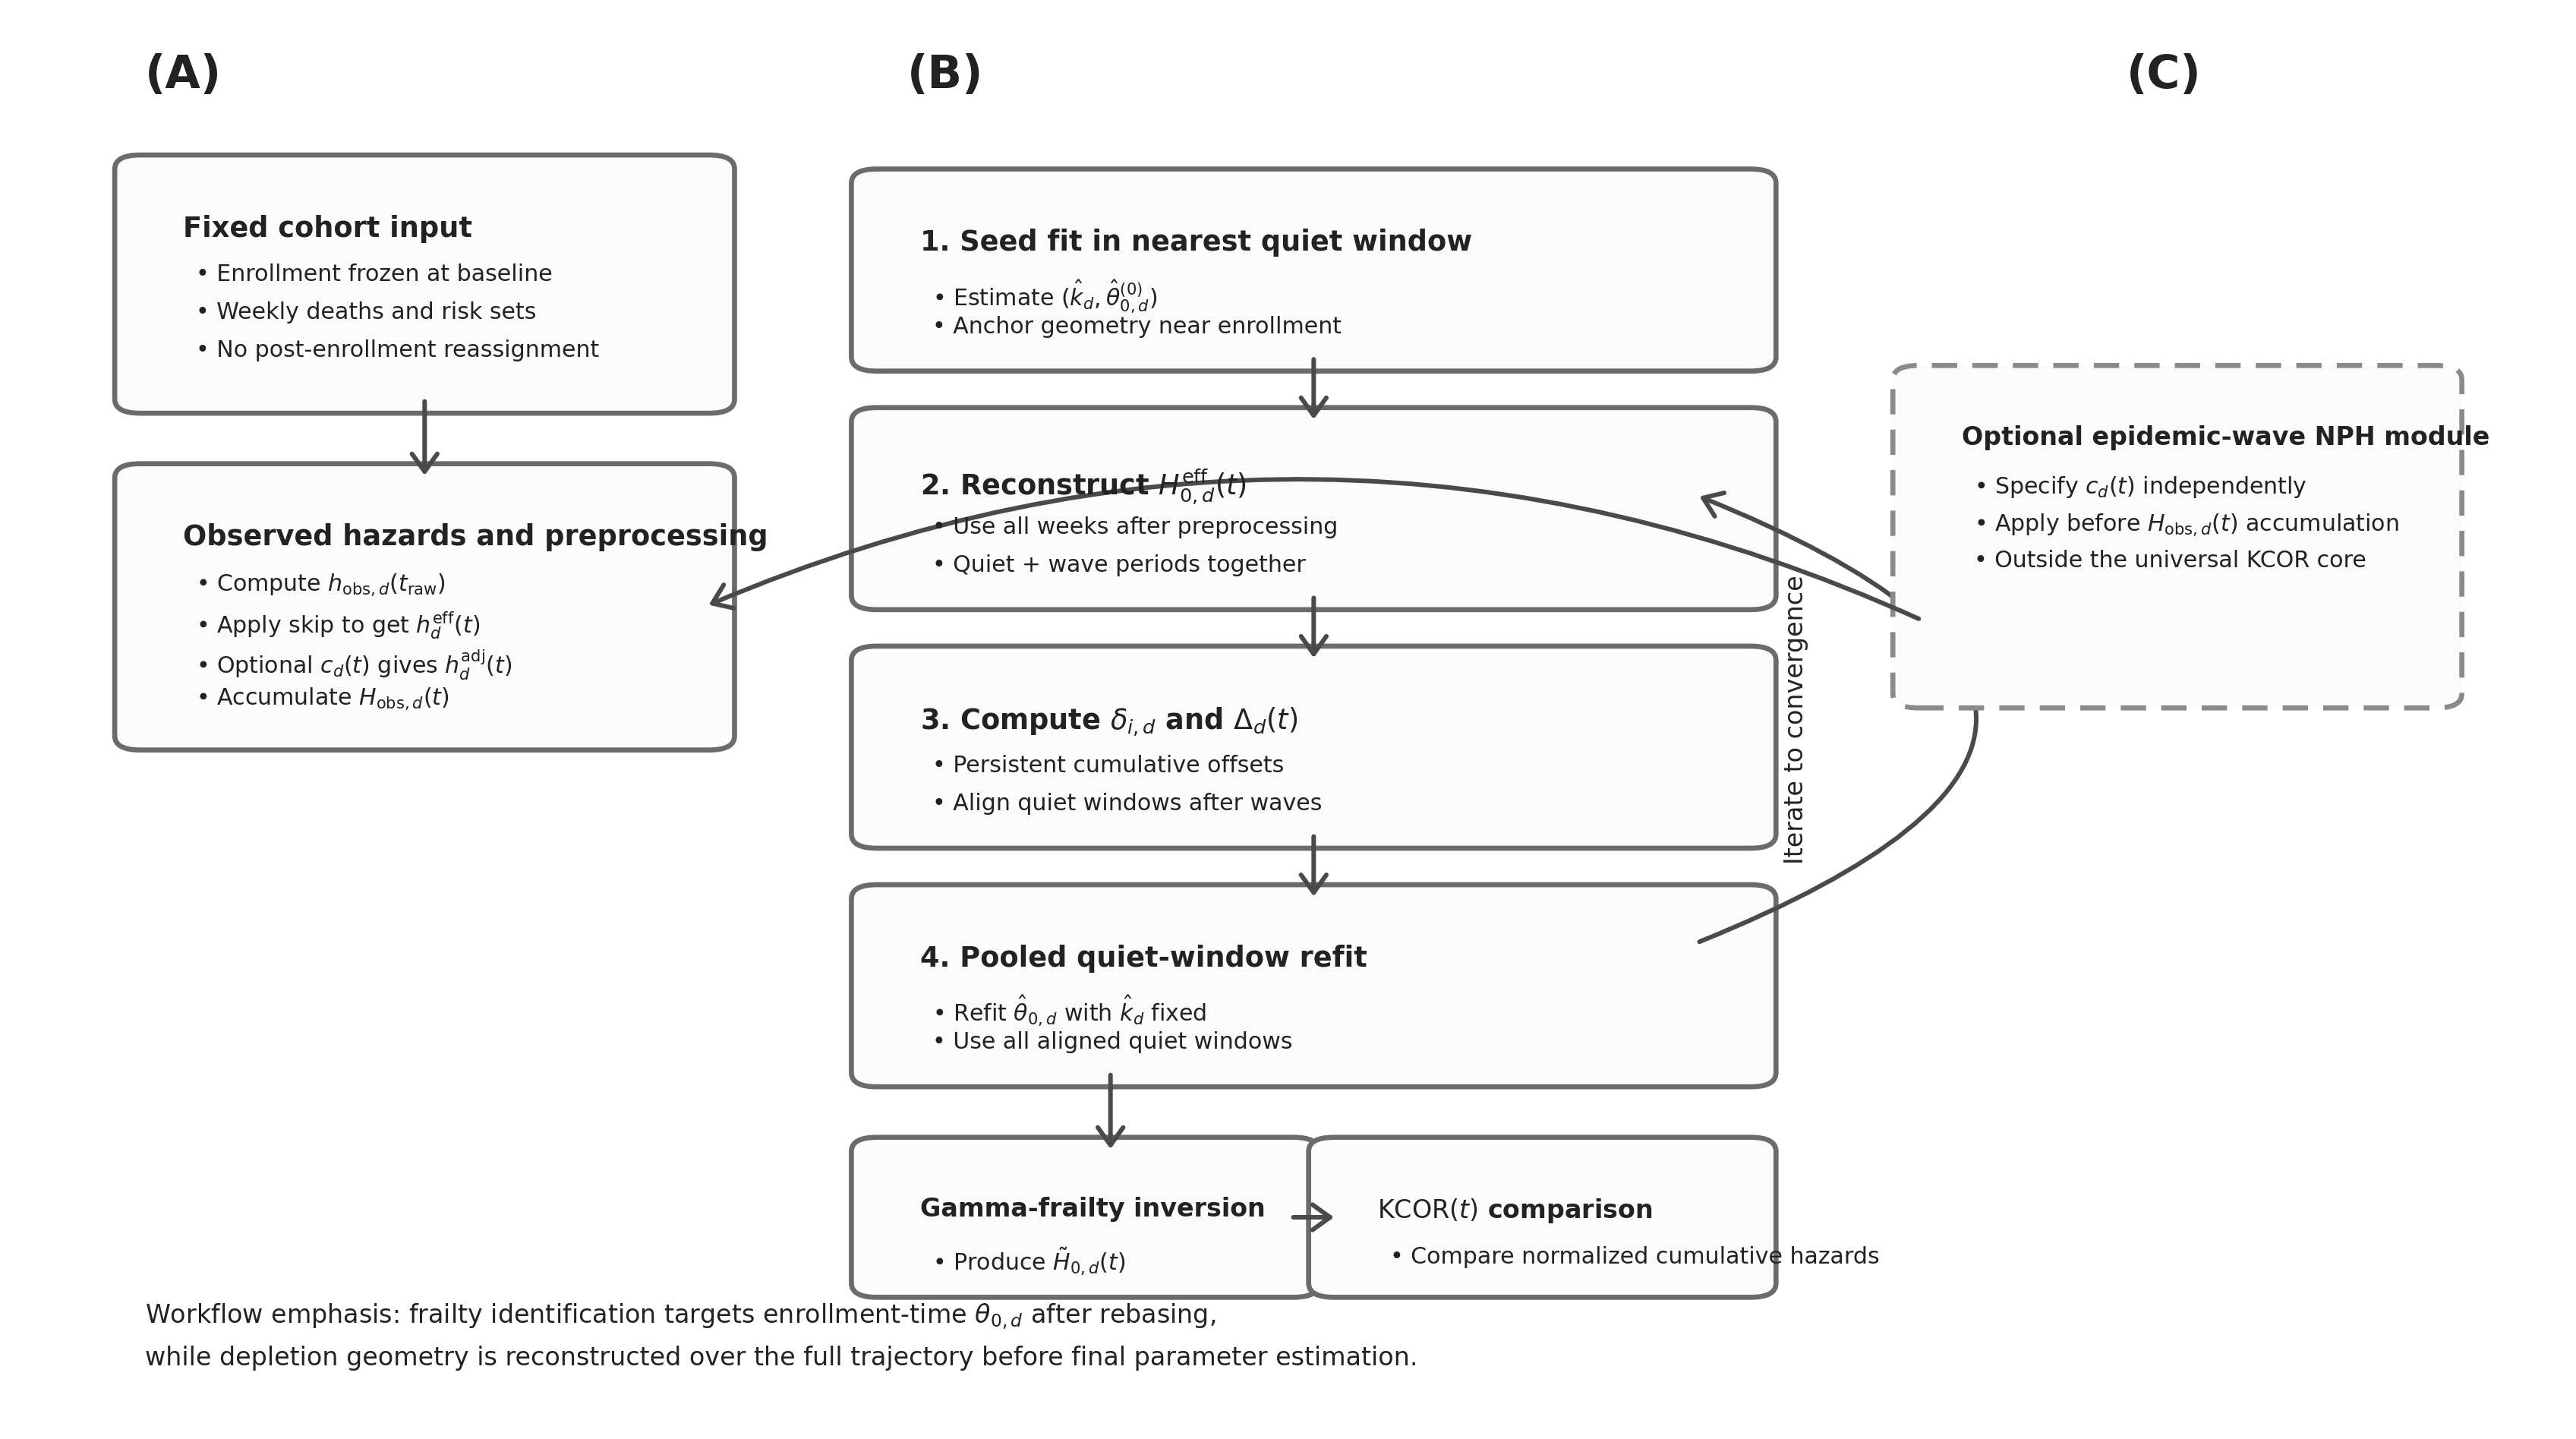
\includegraphics[keepaspectratio,alt={KCOR as a structured four-step estimator. (A) Fixed-cohort cumulative hazards are stabilized after enrollment, and event time is rebased so that frailty identification targets enrollment-time \textbackslash theta\_\{0,d\}. (B) A seed Gompertz fit is obtained in the nearest quiet window, the effective cumulative hazard is reconstructed over the full trajectory, persistent offsets are aligned across quiet windows, and \textbackslash theta\_\{0,d\} is refit jointly before gamma-frailty inversion and KCOR computation. (C) In epidemic-wave applications, an optional NPH extension may adjust wave-period hazards before accumulation and inversion; this extension is not part of the universal KCOR core. This schematic is illustrative rather than empirical. In the schematic, \textbackslash tilde H\_\{0,d\}(t) denotes the depletion-neutralized baseline cumulative hazard and \textbackslash theta\_\{0,d\} denotes enrollment-time frailty variance after the stabilization skip.}]{figures/fig_kcor_workflow.png}}
\caption{\textbf{KCOR as a structured four-step estimator.} \textbf{(A)}
Fixed-cohort cumulative hazards are stabilized after enrollment, and
event time is rebased so that frailty identification targets
enrollment-time \(\theta_{0,d}\). \textbf{(B)} A seed Gompertz fit is
obtained in the nearest quiet window, the effective cumulative hazard is
reconstructed over the full trajectory, persistent offsets are aligned
across quiet windows, and \(\theta_{0,d}\) is refit jointly before
gamma-frailty inversion and KCOR computation. \textbf{(C)} In
epidemic-wave applications, an optional NPH extension may adjust
wave-period hazards before accumulation and inversion; this extension is
not part of the universal KCOR core. \emph{This schematic is
illustrative rather than empirical. In the schematic,
\(\tilde H_{0,d}(t)\) denotes the depletion-neutralized baseline
cumulative hazard and \(\theta_{0,d}\) denotes enrollment-time frailty
variance after the stabilization skip.}}\label{fig:kcor_workflow}
\end{figure}

\subsubsection{2.11 Relationship to Cox proportional
hazards}\label{relationship-to-cox-proportional-hazards}

Cox proportional hazards models estimate an instantaneous hazard ratio
under the assumption that hazards differ by a time-invariant
multiplicative factor. Under selection on frailty with latent
heterogeneity, this assumption is typically violated, yielding
time-varying hazard ratios induced purely by depletion dynamics. This
reflects an estimand mismatch: Cox targets an instantaneous hazard ratio
conditional on survival, whereas KCOR targets a cumulative hazard
contrast after depletion normalization. The resulting Cox failure is
structural (selection plus non-proportional hazards), not a
finite-sample artifact. KCOR operates on Nelson--Aalen--type cumulative
hazards without individual-level frailty observables.

Accordingly, Cox results are presented here as a diagnostic
demonstration of estimand mismatch, not as a competing
intervention-effect estimator. This limitation is consistent with
earlier work by Deeks showing that increasing covariate adjustment in
non-randomized analyses can exacerbate bias and imprecision when
selection effects and measurement error dominate. Deeks further noted
that, despite the widespread reliance on covariate adjustment in
non-randomized studies, there is no empirical evidence that such
adjustment reduces bias on average\textsuperscript{15}.

Even when Cox models are extended with shared frailty to accommodate
heterogeneity, they continue to estimate instantaneous hazard ratios
conditional on survival. KCOR instead uses a cohort-level working model
with Gompertz curvature, enrollment-time \(\theta_0\), and quiet-window
alignment to normalize selection-induced depletion geometry before
computing a cumulative contrast on the depletion-neutralized scale.

\textbf{Distinction from shared-frailty Cox models.}\\
Cox models with shared frailty incorporate unobserved heterogeneity as a
random effect during partial-likelihood maximization, but continue to
estimate an instantaneous hazard ratio conditional on survival. Frailty
variance is treated as a nuisance parameter and depletion geometry is
absorbed into the fitted hazard ratio trajectory. KCOR differs
fundamentally: enrollment-time frailty variance \(\theta_{0,d}\) is
estimated explicitly from aligned quiet-window geometry under a Gompertz
working model and is then analytically inverted \emph{prior} to
comparison. The resulting estimand is a cumulative hazard contrast on a
depletion-neutralized scale, rather than a conditional instantaneous
hazard ratio. Consequently, even when shared-frailty Cox models reduce
bias relative to standard Cox regression, they do not target the same
estimand as KCOR and may still exhibit residual non-null behavior under
selection-only regimes.

\paragraph{2.11.1 Demonstration: Cox bias under frailty heterogeneity
with no treatment
effect}\label{demonstration-cox-bias-under-frailty-heterogeneity-with-no-treatment-effect}

A controlled synthetic experiment was conducted in which the
\textbf{true effect is known to be zero by construction}, isolating
latent frailty heterogeneity as the sole driver of depletion-induced
non-proportional hazards. Cox and KCOR were applied to the same
simulated datasets under identical information constraints.

\textbf{Data-generating process.}

Two cohorts of equal size were simulated under the same baseline hazard
\(h_0(t)\) over time (constant or Gompertz). Individual hazards were
generated as \(z\,h_0(t)\), with frailty \[
z \sim \text{Gamma}(\theta_0^{-1}, \theta_0^{-1}),
\] with mean 1 and variance \(\theta_0\).

Cohort A was generated with \(\theta_0 = 0\) (no frailty heterogeneity),
while Cohort B was generated with \(\theta_0 > 0\). \textbf{No treatment
or intervention effect was applied}: conditional on frailty, the two
cohorts have identical hazards at all times. Thus, the hazard ratio
between cohorts is 1 by construction for all \(t\).

Simulations were repeated over a grid of frailty variances
\(\theta_0 \in \{0, 0.5, 1, 2, 5, 10, 20\}\).

\textbf{Cox analysis.}

For each simulated dataset, a standard Cox proportional hazards model
was fitted using partial likelihood (statsmodels \texttt{PHReg}), with
cohort membership as the sole covariate (no time-varying covariates or
interactions). The resulting hazard ratio estimates and confidence
intervals therefore reflect \textbf{only differences induced by
frailty-driven depletion}, not any treatment effect.

\textbf{KCOR analysis.}

The same simulated datasets were analyzed using KCOR. Observed
cumulative hazards were estimated from cohort-level event counts,
\(\theta_0\) was estimated using the same structured pipeline described
in §2.5, and normalized cumulative hazards were then obtained using Eq.
(\ref{eq:normalized-cumhazard}) prior to computing \(\mathrm{KCOR}(t)\).
Although the data-generating process specifies individual hazards, the
KCOR analysis mirrors the aggregated information available in registry
studies rather than exploiting simulator-only knowledge.
Post-normalization slope and asymptotic \(\mathrm{KCOR}(t)\) values were
examined as one component of the broader validation stack rather than as
the sole validation criterion.

\textbf{Expected behavior under the null.}

Because the data-generating process includes \textbf{no treatment
effect}, any valid estimator should return a null result. In this
setting:

\begin{itemize}
\tightlist
\item
  \textbf{Cox regression} is expected to produce apparent non-null
  hazard ratios as \(\theta_0\) increases, reflecting differential
  selection-induced depletion and violation of proportional hazards
  induced by frailty heterogeneity.
\item
  \textbf{KCOR} is expected to remain centered near unity with
  negligible post-normalization slope across all \(\theta_0\),
  consistent with correct null behavior after depletion normalization.
\end{itemize}

\textbf{Summary of findings.}

Across increasing values of \(\theta_0\), Cox regression produced
progressively larger apparent deviations from a hazard ratio of 1. The
direction and magnitude of the apparent effect depended on the follow-up
horizon and degree of frailty heterogeneity. In contrast,
\(\mathrm{KCOR}(t)\) trajectories remained stable and centered near
unity, with post-normalization slopes approximately zero across all
simulated conditions.

These results indicate that \textbf{frailty heterogeneity alone is
sufficient to induce spurious hazard ratios in Cox regression}, while
KCOR returns a null result under the same conditions.

Table \ref{tbl:cox_bias_demo} reports numerical summaries of the
Cox-vs-KCOR behavior across the frailty grid. Small residual deviations
in the asymptotic level are expected under extreme frailty heterogeneity
and are negligible relative to the distortions observed under Cox; the
diagnostic criterion is slope stability rather than exact unity.

Additional Cox HR results from the same synthetic-null grid are shown in
Figure \ref{fig:cox_bias_hr}.

A compact summary of KCOR bias as a function of frailty variance
\(\theta_0\) is provided in the Supplementary Information (Figure
\ref{fig:si_kcor_bias_vs_theta}).

\begin{figure}
\centering
\pandocbounded{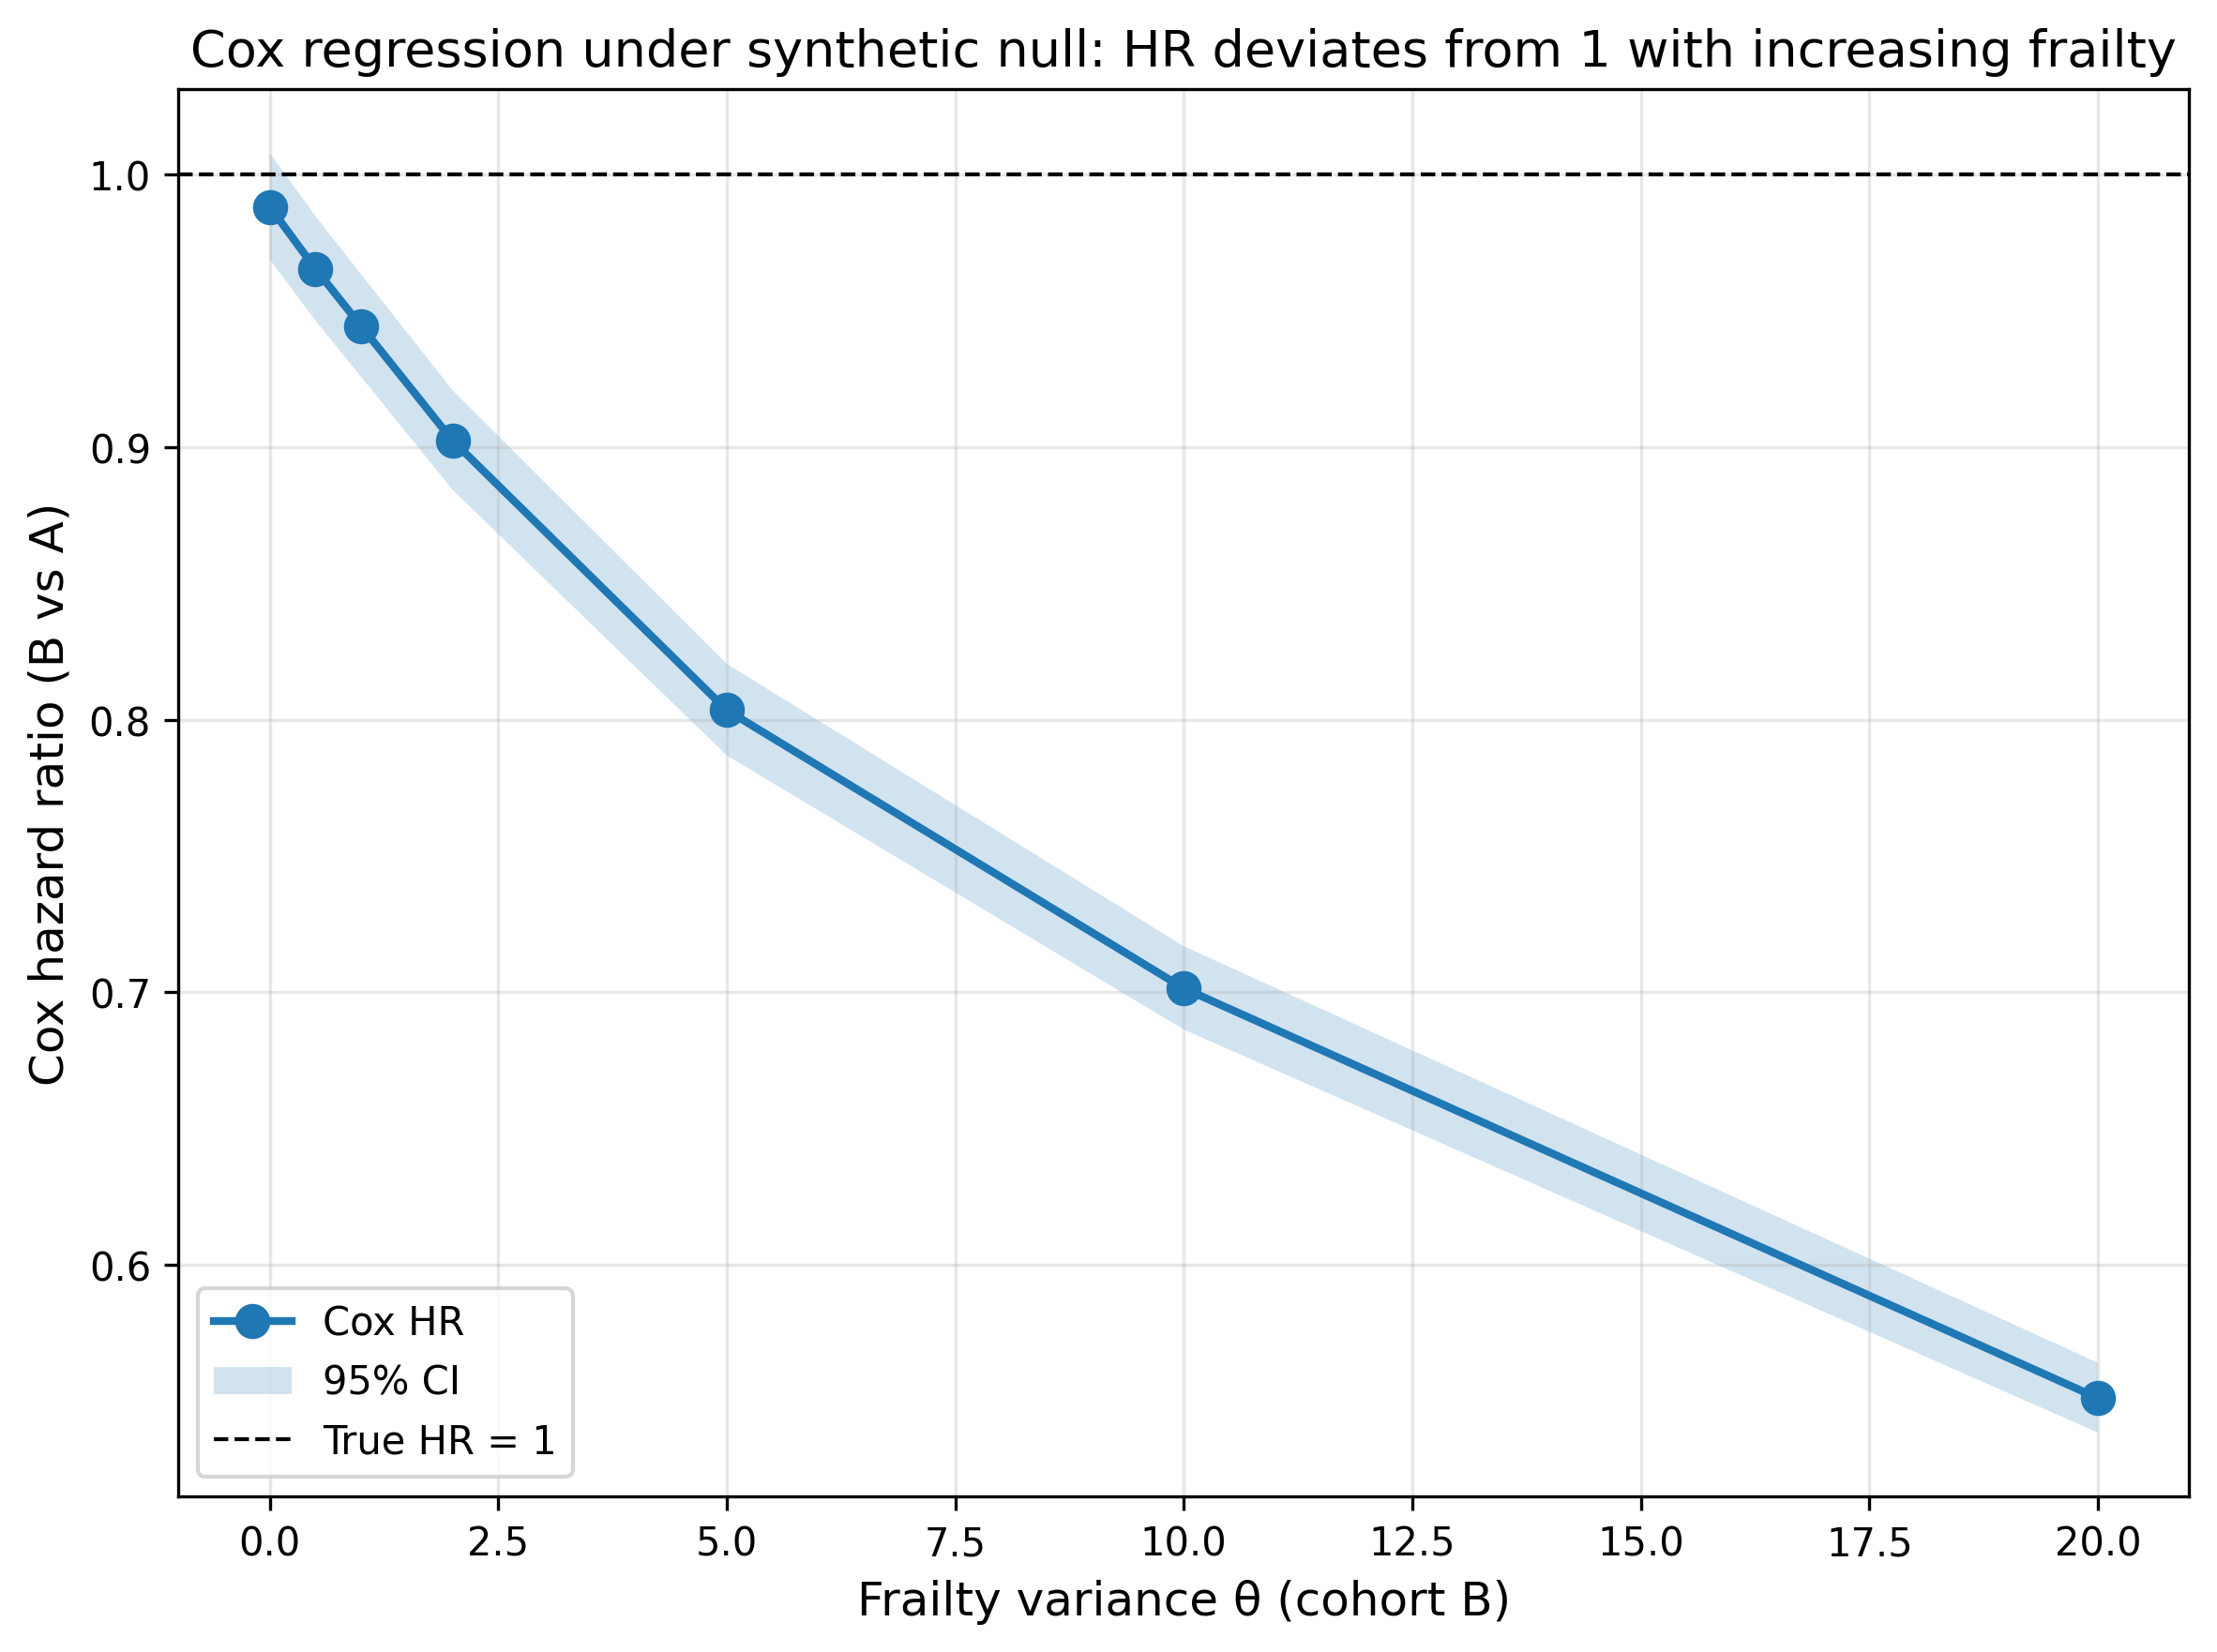
\includegraphics[keepaspectratio,alt={Cox regression produces spurious non-null hazard ratios under a synthetic null as frailty heterogeneity increases. Hazard ratios (with 95\% confidence intervals) from Cox proportional hazards regression comparing cohort B to cohort A in simulations where the true treatment effect is identically zero and cohorts differ only in enrollment-time frailty variance (\textbackslash theta\_0). Deviations from HR=1 arise solely from frailty-driven depletion and associated non-proportional hazards.}]{figures/fig_cox_bias_hr_vs_theta.png}}
\caption{Cox regression produces spurious non-null hazard ratios under a
\emph{synthetic null} as frailty heterogeneity increases. Hazard ratios
(with 95\% confidence intervals) from Cox proportional hazards
regression comparing cohort B to cohort A in simulations where the true
treatment effect is identically zero and cohorts differ only in
enrollment-time frailty variance (\(\theta_0\)). Deviations from HR=1
arise solely from frailty-driven depletion and associated
non-proportional hazards.}\label{fig:cox_bias_hr}
\end{figure}

\begin{figure}
\centering
\pandocbounded{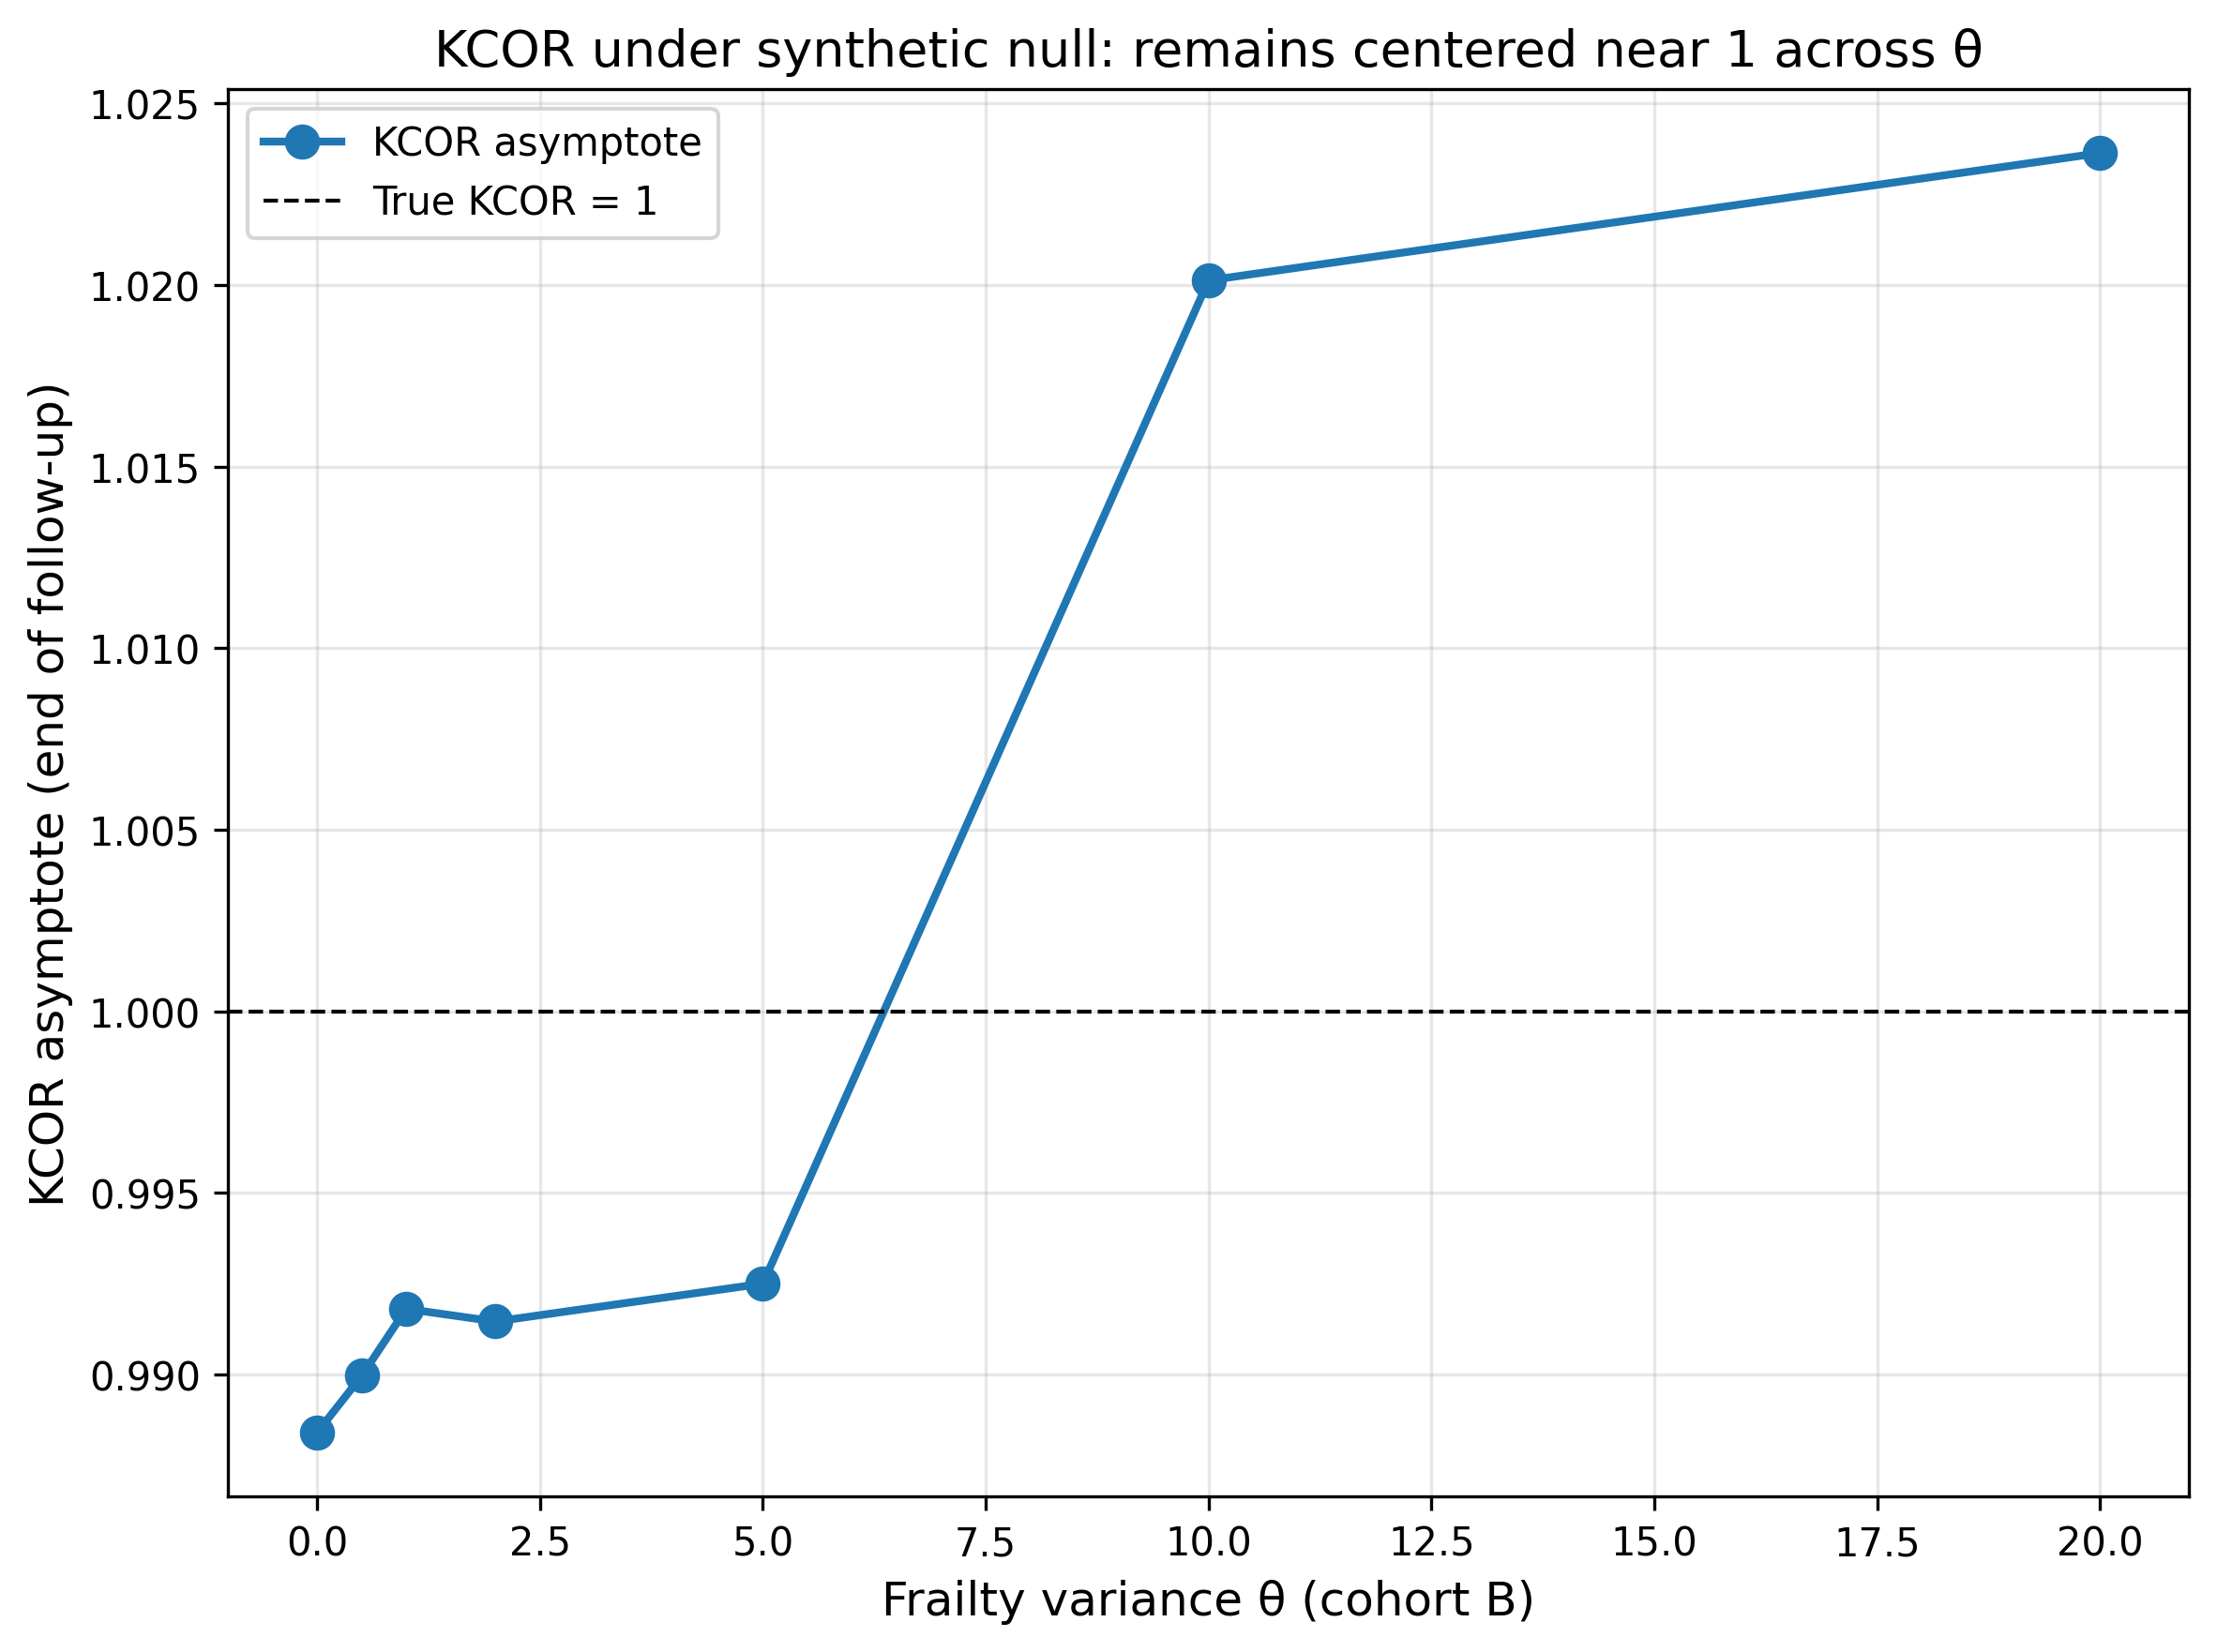
\includegraphics[keepaspectratio,alt={\textbackslash mathrm\{KCOR\}(t) remains null under a synthetic null across increasing frailty heterogeneity. \textbackslash mathrm\{KCOR\}(t) asymptotes remain near 1 across \textbackslash theta\_0 in the same simulations, consistent with correct null behavior after depletion normalization. Uncertainty bands (95\% bootstrap intervals) are shown but are narrow due to large sample sizes.}]{figures/fig_cox_bias_kcor_vs_theta.png}}
\caption{\(\mathrm{KCOR}(t)\) remains null under a synthetic null across
increasing frailty heterogeneity. \(\mathrm{KCOR}(t)\) asymptotes remain
near 1 across \(\theta_0\) in the same simulations, consistent with
correct null behavior after depletion normalization. Uncertainty bands
(95\% bootstrap intervals) are shown but are narrow due to large sample
sizes.}\label{fig:cox_bias_kcor}
\end{figure}

\textbf{Interpretation.}

This controlled synthetic null indicates that Cox proportional hazards
regression can report highly statistically significant non-null hazard
ratios even when the true effect is identically zero, purely due to
frailty-driven depletion and induced non-proportional hazards. KCOR
remains near unity under the same conditions because depletion
normalization precedes comparison.

\subsubsection{2.12 Worked example
(descriptive)}\label{worked-example-descriptive}

A brief worked example is included to illustrate the KCOR workflow
end-to-end. This example is descriptive and intended solely to
illustrate the mechanics of cohort construction, hazard estimation,
\(\theta_0\) estimation, depletion normalization, and KCOR computation.

The example proceeds from aggregated cohort counts through
cumulative-hazard estimation, stabilization and rebasing,
delta-iteration fitting across prespecified quiet windows, gamma
inversion, and \(\mathrm{KCOR}(t)\) construction, accompanied by
diagnostic plots assessing post-normalization linearity and parameter
stability.

\subsubsection{2.13 Reproducibility and computational
implementation}\label{reproducibility-and-computational-implementation}

All figures, tables, and simulations can be reproduced from the
accompanying code repository. The manuscript is built from
\texttt{documentation/preprint/paper.md} using the root
\texttt{Makefile} paper target \texttt{make\ paper-full}.

Additional environment and runtime details are provided in the
Supplementary Information (SI); code and archival links are provided in
Code/Data Availability.

\subsubsection{2.14 Data requirements and feasible study
designs}\label{data-requirements-and-feasible-study-designs}

KCOR is designed for settings where outcomes are ascertained repeatedly
over time but individual-level covariates, visit schedules, or
counterfactual exposure histories are unavailable or unreliable. This
section clarifies the data structures required for valid application, as
well as designs for which the method is not appropriate.

\textbf{Minimum data requirements.} KCOR requires (i) a well-defined
cohort entry or enrollment rule, (ii) repeated outcome ascertainment
over calendar or follow-up time (which may be passive), (iii) sufficient
event counts to estimate cumulative hazards with reasonable stability,
and (iv) the presence of at least one diagnostically identifiable
``quiet'' window during which baseline risk is approximately stable.
Individual-level covariates, treatment assignment models, or visit-based
follow-up schedules are not required.

\textbf{What KCOR does not require.} Unlike causal estimators,
interrupted time-series methods, synthetic controls, or digital twin
approaches, KCOR does not require exchangeability assumptions,
individual-level confounder measurement, continuous exposure tracking,
or explicit modeling of counterfactual untreated trajectories. The
method operates entirely on aggregated cumulative hazard information and
is therefore compatible with registries and administrative systems where
outcomes are captured far more frequently than exposures or visits.

\textbf{Well-suited data sources and designs.} KCOR is particularly well
matched to vital statistics--linked cohorts, administrative or
registry-based studies with passive outcome capture, program enrollments
with irregular follow-up but reliable endpoints, and population-based
datasets where cohorts are defined by eligibility, vulnerability, or
sociodemographic characteristics rather than repeated clinical
encounters.

\textbf{Designs where KCOR is not appropriate.} KCOR is not suitable for
settings with extremely sparse events, rapidly shifting baseline hazards
with no diagnostically quiet interval, highly fluid cohorts with
frequent switching between exposure groups, or outcome ascertainment
that is strictly conditional on clinic visits. In such cases, the
required identifiability diagnostics will fail and results should not be
reported.

\subsection{3. Results}\label{results}

This section evaluates the revised KCOR estimator in four layers: (i)
recovery of enrollment-time frailty variance \(\theta_0\) and
corresponding null behavior in synthetic settings, (ii) empirical
negative controls, (iii) positive controls with injected effects, and
(iv) failure signaling under model stress. Synthetic-null flatness
remains informative, but it is no longer the sole validation anchor.

The central validation claim is therefore broader than in earlier
versions of the paper:

\begin{itemize}
\tightlist
\item
  \textbf{Identification performance:} the estimator should recover
  \(\theta_0\) and align quiet windows coherently under the stated
  working model.
\item
  \textbf{Negative-control behavior:} under a true null effect, KCOR
  should remain approximately flat at 1 after normalization, subject to
  sampling variability.
\item
  \textbf{Positive-control behavior:} when known harm/benefit is
  injected, KCOR should deviate in the expected direction after the same
  normalization pipeline.
\item
  \textbf{Failure signaling:} when key assumptions are violated or the
  working model is stressed, diagnostics should degrade and the analysis
  should be treated as not identified rather than reported as a stable
  contrast.
\end{itemize}

Throughout, curvature in cumulative-hazard plots reflects
selection-induced depletion or external hazard structure, while
linearity after normalization within quiet windows is interpreted as a
diagnostic consistency check rather than as a proof that all confounding
has been removed.

In vaccinated--unvaccinated comparisons, large early differences in
\(\mathrm{KCOR}(t)\) may reflect baseline risk selection rather than
intervention-attributable effects; in such cases,
\(\mathrm{KCOR}(t; t_0)\) is emphasized to report deviations relative to
an early post-enrollment reference while preserving time-varying
divergence.

\subsubsection{3.1 Negative controls (selection-only
null)}\label{negative-controls-selection-only-null}

\paragraph{\texorpdfstring{3.1.1 Structured synthetic validation:
\(\theta_0\) recovery and null
behavior}{3.1.1 Structured synthetic validation: \textbackslash theta\_0 recovery and null behavior}}\label{structured-synthetic-validation-theta_0-recovery-and-null-behavior}

We first evaluate KCOR under synthetic settings in which the
data-generating process matches the revised working model. The primary
synthetic target is no longer only whether \(\mathrm{KCOR}(t)\) is flat
under a null; it is also whether the estimator recovers the
\textbf{enrollment-time} frailty variance \(\theta_0\) that generated
the cohort geometry.

Under correct specification, the revised estimator should recover
\(\theta_0\) with small error, align the quiet windows coherently after
offset reconstruction, and then produce \(\mathrm{KCOR}(t)\)
trajectories that remain approximately constant at 1 under a true null
effect. Full design details, recovery grids, and figures are provided in
the Supplementary Information, including the \(\theta_0\) recovery
simulations and the synthetic negative-control figures (Section S4.2.1
and related figures).

\paragraph{3.1.2 Empirical negative control using national registry data
(Czech
Republic)}\label{empirical-negative-control-using-national-registry-data-czech-republic}

This application is presented solely to illustrate KCOR's diagnostic
behavior on real registry data; it uses an age-shift construction
(pseudo-cohorts) that is a negative control by design rather than an
observational treatment-effect analysis. No causal interpretation of
vaccine effects is implied.

The repository includes a pragmatic negative control construction that
repurposes a real dataset by comparing ``like with like'' while inducing
large composition differences (e.g., age band shifts). In this
construction, age strata are remapped into pseudo-doses so that
comparisons are, by construction, within the same underlying category;
the expected differential contrast is near zero, but the baseline
hazards differ strongly.

These age-shift negative controls deliberately induce extreme baseline
mortality differences (10--20 year age gaps) while preserving a
pseudo-null by construction, since all vaccination states are compared
symmetrically. The \(\mathrm{KCOR}(t)\) trajectories are expected to be
horizontal under the null, subject to sampling stochasticity, consistent
with the estimator normalizing selection-induced depletion curvature
without introducing spurious time trends or cumulative drift. This is an
empirical negative control of \textbf{end-to-end behavior}, not a proof
that every source of confounding has been removed.

For the empirical age-shift negative control (Figure
\ref{fig:neg_control_10yr}), aggregated weekly cohort summaries derived
from the Czech Republic administrative mortality and vaccination dataset
are used and exported in KCOR\_CMR format.

Notably, KCOR estimates frailty parameters independently for each cohort
without knowledge of exposure status; the observed asymmetry in
depletion normalization arises entirely from differences in hazard
curvature rather than from any vaccination-specific assumptions.

Figure \ref{fig:neg_control_10yr} provides a representative
illustration; additional age-shift variants are provided in the
Supplementary Information (SI).

\begin{figure}
\centering
\pandocbounded{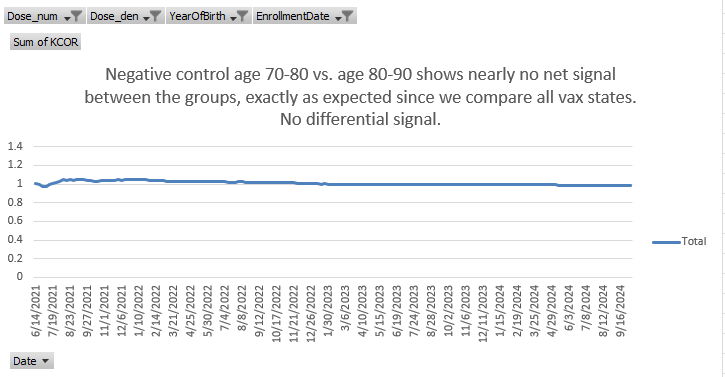
\includegraphics[keepaspectratio,alt={Empirical negative control with approximately 10-year age difference between cohorts. Despite large baseline mortality differences, \textbackslash mathrm\{KCOR\}(t) is expected to be horizontal under the null, subject to sampling stochasticity, consistent with the pseudo-null construction. Curves are shown as anchored \textbackslash mathrm\{KCOR\}(t; t\_0), i.e., \textbackslash mathrm\{KCOR\}(t)/\textbackslash mathrm\{KCOR\}(t\_0), which removes pre-existing cumulative differences and displays post-anchor divergence only. KCOR curves are anchored at t\_0 = 4 weeks (i.e., plotted as \textbackslash mathrm\{KCOR\}(t; t\_0)). Cumulative hazard is indexed from week 4 following enrollment. Uncertainty bands (95\% bootstrap intervals) are shown. Data source: Czech Republic mortality and vaccination dataset processed into KCOR\_CMR aggregated format (negative-control construction; see Supplementary Information (SI)).}]{figures/fig2_neg_control_10yr_age_diff.png}}
\caption{Empirical negative control with approximately 10-year age
difference between cohorts. Despite large baseline mortality
differences, \(\mathrm{KCOR}(t)\) is expected to be horizontal under the
null, subject to sampling stochasticity, consistent with the pseudo-null
construction. Curves are shown as anchored \(\mathrm{KCOR}(t; t_0)\),
i.e., \(\mathrm{KCOR}(t)/\mathrm{KCOR}(t_0)\), which removes
pre-existing cumulative differences and displays post-anchor divergence
only. KCOR curves are anchored at \(t_0 = 4\) weeks (i.e., plotted as
\(\mathrm{KCOR}(t; t_0)\)). Cumulative hazard is indexed from week 4
following enrollment. Uncertainty bands (95\% bootstrap intervals) are
shown. Data source: Czech Republic mortality and vaccination dataset
processed into KCOR\_CMR aggregated format (negative-control
construction; see Supplementary Information
(SI)).}\label{fig:neg_control_10yr}
\end{figure}

Table \ref{tbl:neg_control_summary} provides numeric summaries.

\subsubsection{3.2 Positive controls (injected
effects)}\label{positive-controls-injected-effects}

Positive controls (injected harm/benefit) are provided in Supplementary
Section S3. They verify that after the same preprocessing and
\(\theta_0\) estimation pipeline, KCOR deviates in the expected
direction and with magnitude consistent with the injected effect (up to
discretization and sampling noise).

In positive-control simulations with injected multiplicative hazard
shifts, KCOR reliably detects both harm and benefit, with estimated
\(\mathrm{KCOR}(t)\) trajectories tracking the imposed effects. This
complements the null validations by showing that the revised estimator
is not merely flattening trajectories indiscriminately; it can also
preserve true post-normalization divergence when an effect is present.

\subsubsection{3.3 Stress tests (frailty
misspecification)}\label{stress-tests-frailty-misspecification}

\paragraph{3.3.1 Frailty misspecification
robustness}\label{frailty-misspecification-robustness}

To assess robustness to departures from the gamma frailty assumption,
simulations were conducted under alternative frailty distributions while
maintaining the same selection-induced depletion geometry. These stress
tests also probe the new estimator's vulnerability to failure of the
offset structure, weak curvature, and model overfit. Simulations were
performed for:

\begin{itemize}
\tightlist
\item
  \textbf{Gamma} (baseline reference)
\item
  \textbf{Lognormal} frailty
\item
  \textbf{Two-point mixture} (discrete frailty)
\item
  \textbf{Bimodal} frailty distributions
\item
  \textbf{Correlated frailty} (within-subgroup correlation)
\end{itemize}

For each frailty specification, bias (deviation from true cumulative
hazard ratio), variance (trajectory stability), coverage (proportion of
simulations where uncertainty intervals contain the true value), and
non-identifiability rate (proportion of simulations where diagnostics
indicated non-identifiability) are reported.

Under frailty misspecification, KCOR can degrade gracefully by
attenuating toward unity or by not meeting diagnostic criteria, rather
than producing spurious large effects. When the alternative frailty
distribution produces similar depletion geometry to gamma frailty, KCOR
normalization remains approximately valid, with bias remaining small and
diagnostics indicating successful identification. When the alternative
frailty structure produces substantially different depletion geometry,
or when the structured offset model fails to align windows coherently,
diagnostics (poor fit, residual structure, offset instability, or weak
identification) correctly signal that the working approximation is
inadequate. The pathological/non-gamma frailty mixture simulation in the
Supplement provides a concrete stress test of this regime.

\paragraph{3.3.2 Quiet-window contamination stress
test}\label{quiet-window-contamination-stress-test}

Positive controls inject multiplicative hazard shifts in an effect window
to test whether KCOR detects a true contrast. A distinct concern is
whether non-frailty curvature confined to a quiet window could bias
\(\hat\theta_{0}\) enough to shift anchored KCOR away from a true null.
We therefore ran a synthetic experiment with known \(\theta_{0}\)
(Gompertz-plus-gamma-frailty DGP, two cohorts with the same baseline scale
\(k\) calibrated to Czech KCOR\_CMR weekly hazard for 1940--1960, dose 0
reference) and additive contamination applied only to the lower-frailty
cohort during rebased weeks 4--56. Types tested: decaying dynamic-style
hazard, constant comorbidity-style hazard, and their joint \(4\times4\)
grid on strictly positive amplitudes. Each setting used 20 stochastic
replicates; the production pipeline (\texttt{fit\_theta0\_gompertz},
inversion, anchored KCOR as in the simulation grid) was applied per
replicate. Key outputs:
\texttt{test/quiet\_window\_contamination/out/quiet\_contamination\_agg.csv},
\texttt{fig\_quiet\_contam\_theta\_error.png} (mean
\(\hat\theta_{0,A}\) error vs.\ \(\epsilon\) for the 1D sweeps; the
\textbf{combined} panel is a heatmap of the fraction of replicates with
anchored \(\mathrm{KCOR}_\infty>1\) on the \(4\times4\) joint grid),
\texttt{fig\_quiet\_contam\_kcor\_asymptote.png}; the script prints a
one-line combined sign-reversal summary for the joint grid. Full
per-replicate rows are in \texttt{quiet\_contamination\_long.csv}.
Interpret contamination magnitudes alongside \(h_{\mathrm{ref}}\) and
\(\epsilon/h_{\mathrm{ref}}\) reported in those tables.

Additional validation results---including full simulation grids, quiet-window
robustness catalogs, dynamic-selection checks, and extended comparator
analyses---are provided in the Supplementary Information (SI).

Additional derivations, simulation studies, robustness analyses, and
implementation details are provided in the Supplementary Information.

\subsection{4. Discussion}\label{discussion}

\subsubsection{4.1 Limits of attribution and
non-identifiability}\label{limits-of-attribution-and-non-identifiability}

A notable strength of this study is the use of publicly available,
record-level national mortality data, which permits independent
verification and replication without reliance on restricted registries.

KCOR should be viewed as complementary to hazard-based modeling rather
than as a substitute. Cox models and flexible parametric approaches
estimate instantaneous hazard relationships and allow time-varying
coefficients, whereas KCOR addresses cumulative survival curvature
arising from frailty-induced depletion. When depletion geometry
materially distorts marginal hazard ratios, KCOR provides an alternative
summary contrast at the cumulative scale.

KCOR does not uniquely identify the biological, behavioral, or clinical
mechanisms responsible for observed hazard heterogeneity. In particular,
curvature in the cumulative hazard may arise from multiple sources,
including selection on latent frailty, behavior change, seasonality,
treatment effects, reporting artifacts, or their combination. Depletion
of susceptibles is therefore used as a parsimonious working model whose
adequacy is evaluated through diagnostics and negative controls, rather
than assumed as a substantive truth. KCOR's estimand is whether a
cumulative outcome contrast persists after removal of curvature
consistent with the working depletion model, not attribution of that
curvature to a specific mechanism. \textbf{Identifiability under the
revised estimator.}\\
Even under ideal data quality, KCOR does not identify \(\theta_0\) from
an arbitrary mortality trajectory. Identification now depends on a joint
regime: a plausible Gompertz baseline, a well-defined rebased origin
after the stabilization skip, sufficient curvature to distinguish
\(k_d\) from \(\theta_{0,d}\), quiet windows that remain coherent after
alignment, and a structured cumulative-hazard offset model when the
delta path is used. If any of these conditions fails, the estimator is
weakly identified or non-identified.

This ambiguity remains structural rather than cosmetic. In minimal
aggregated data, depletion-induced curvature, constant proportional
hazard shifts, and external time-varying hazards are not generically
separable over short horizons. The revised estimator improves internal
coherence by aligning the parameter target with enrollment time and by
pooling information across quiet windows, but it does not eliminate the
need for diagnostics or transform the method into a causal effect
estimator.

\subsubsection{4.2 What KCOR estimates}\label{what-kcor-estimates}

\emph{Table \ref{tbl:positioning} clarifies that KCOR differs from
non-proportional hazards methods not in flexibility, but in estimand and
direction of inference.} KCOR normalizes selection-induced depletion and
then compares depletion-neutralized cumulative hazards;
\(\mathrm{KCOR}(t)\) summarizes cumulative outcome accumulation rather
than instantaneous hazard ratios. It is descriptive rather than causal,
and interpretability is conditional on the stated assumptions and
prespecified diagnostics (seed-fit quality, post-normalization
linearity, multi-window consistency, and parameter stability). When
diagnostics fail, contrasts are not reported and results are treated as
non-identifiable rather than as substantive cumulative effects. Anchored
KCOR is used only when explicitly stated to remove pre-existing level
differences and emphasize post-reference divergence.

Cumulative contrasts are particularly informative in settings where
early hazard ratios attenuate over time due to depletion of high-risk
individuals, leading instantaneous hazard-based summaries to obscure
long-horizon risk differences.

\subsubsection{4.3 Relationship to negative control
methods}\label{relationship-to-negative-control-methods}

Negative control outcomes/tests are widely used to \emph{detect}
confounding. KCOR's objective is different: it is an estimator intended
to \emph{normalize away a specific confounding
structure}---selection-induced depletion dynamics---prior to comparison.
Negative and positive controls are nevertheless central to validating
the estimator's behavior.

This asymmetry helps explain why standard observational analyses can
show large mortality differences during periods lacking a plausible
mechanism: vaccinated cohorts are already selection-filtered, while
unvaccinated hazards are suppressed by ongoing frailty depletion.
Unadjusted comparisons therefore systematically understate unvaccinated
baseline risk and exaggerate apparent differences.

\subsubsection{4.4 Practical guidelines for
implementation}\label{practical-guidelines-for-implementation}

This subsection summarizes common operational practices for applying
KCOR in retrospective cohort studies and for assessing when resulting
contrasts are interpretable.

Reporting commonly includes:

\begin{itemize}
\tightlist
\item
  Enrollment definition and justification
\item
  Risk set definitions and event-time binning
\item
  Quiet-window definitions and justification across all windows used for
  \(\theta_0\) identification
\item
  Gompertz baseline choice, rebased time origin, and fit diagnostics for
  \(\theta_0\)
\item
  Skip/stabilization rule and robustness to nearby values
\item
  Delta-offset diagnostics and multi-window consistency checks
\item
  If used, rationale and diagnostics for the optional epidemic-wave NPH
  extension
\item
  Predefined negative/positive controls used for validation
\item
  Sensitivity analysis plan and results
\end{itemize}

KCOR should therefore be applied and reported as a complete
pipeline---from cohort freezing, through depletion normalization, to
cumulative comparison and diagnostics---rather than as a standalone
adjustment step. Scope and interpretation are summarized once in Box 2
(§1.6).

KCOR is diagnostic-first: multiplicity concerns are mitigated by
prespecification of cohorts, quiet windows, and control constructions.
Exploratory stratified analyses should be interpreted descriptively,
with emphasis on diagnostic consistency rather than formal significance
claims.

\subsection{5. Limitations}\label{limitations}

This section summarizes the principal limitations of the KCOR framework,
emphasizing conditions under which interpretation is restricted rather
than situations in which the estimator fails. These limitations are
diagnostic and design-related, reflecting the framework's intentionally
conservative scope.

KCOR is intentionally diagnostic rather than test-based: it does not
attempt to formally test properties such as quiet-window validity or
frailty distributional form, but instead enforces conservative
interpretability gates when prespecified empirical diagnostics fail.
KCOR is not a causal effect estimator and does not identify
counterfactual outcomes under hypothetical interventions.

KCOR does not guarantee nominal uncertainty calibration under arbitrary
frailty misspecification. Because the gamma frailty model is used as a
working approximation, confidence intervals may be mildly
anti-conservative in sparse-event regimes or when depletion geometry
deviates substantially from gamma. Diagnostic criteria are intended to
identify such regimes; estimates from failing windows should not be
interpreted.

\begin{itemize}
\tightlist
\item
  \textbf{Model dependence}: Normalization relies on the adequacy of the
  gamma-frailty model, the Gompertz baseline assumption, and the
  structured offset logic used to align quiet windows.
\item
  \textbf{Relation to existing non-PH methods}: KCOR is complementary to
  time-varying Cox, flexible parametric, additive hazards, and MSM
  approaches; these methods address different estimands and
  identification strategies, whereas KCOR targets depletion-geometry
  normalization under minimal-data constraints (see §1.3.1).
\item
  \textbf{\(\theta_0\) estimation is data-derived}: KCOR does not impose
  \(\theta_0 = 0\) for any cohort. Near-zero fitted \(\theta_0\) values
  indicate weak identifiability or minimal detectable depletion
  curvature under the working model and should not be interpreted as an
  assumption of cohort homogeneity.
\item
  \textbf{Sparse events}: When event counts are small, hazard estimation
  and parameter fitting can be unstable.
\item
  \textbf{Contamination of quiet periods}: External shocks (e.g.,
  epidemic waves) overlapping the quiet window can bias
  selection-parameter estimation.
\item
  \textbf{Applicability to other outcomes}: Although this paper focuses
  on all-cause mortality, KCOR is applicable to other irreversible
  outcomes provided that event timing and risk sets are well defined.
  Application to cause-specific mortality would require explicit
  competing-risk definitions and cause-specific hazards, but the
  normalization logic remains cumulative and descriptive. Extension to
  non-fatal outcomes such as hospitalization is conceptually
  straightforward but may require additional attention to outcome
  definitions, censoring mechanisms, and recurrent events. These
  considerations affect interpretation rather than the core KCOR
  framework.
\item
  \textbf{Non-gamma frailty}: The KCOR framework assumes that selection
  acts approximately multiplicatively through a time-invariant frailty
  distribution, for which the gamma family provides a convenient and
  empirically testable approximation. In settings where depletion
  dynamics are driven by more complex mechanisms---such as time-varying
  frailty variance, interacting risk factors, or shared frailty
  correlations within subgroups---the curvature structure exploited by
  KCOR may be misspecified. In such cases, KCOR diagnostics (e.g., poor
  curvature fit or unstable fitted frailty variance estimates) serve as
  indicators of model inadequacy rather than targets for parameter
  tuning. Extending the framework to accommodate dynamic or correlated
  frailty structures would require explicit model generalization rather
  than modification of KCOR normalization steps and is left to future
  work. Empirically, KCOR's validity depends on curvature removal rather
  than the specific parametric form; alternative frailty distributions
  that generate similar depletion geometry would yield equivalent
  normalization.
\end{itemize}

Sensitivity analyses in this work are intentionally embedded alongside
the assumptions they interrogate, rather than consolidated into a single
omnibus robustness section. Parameters governing quiet-window
identification, frailty normalization, aggregation, and uncertainty
estimation are stress-tested through targeted negative controls,
pathological simulations, and diagnostic failure demonstrations. This
structure reflects the diagnostic-first philosophy of KCOR: robustness
is assessed by whether assumptions remain identifiable and diagnostics
pass, not by tuning parameters to stabilize point estimates.

\textbf{Interpretation of sub-nominal bootstrap coverage}

Table \ref{tbl:bootstrap_coverage} reports empirical coverage using the
per-dataset bootstrap design described in the table caption (each simulated
dataset yields its own percentile interval; coverage is the fraction of
datasets for which the true $\mathrm{KCOR}(t)$ at the evaluation week lies
inside that interval). \textbf{Under frailty misspecification or sparse-event
regimes, one generally expects sub-nominal empirical coverage for
working-model percentile intervals at sufficient Monte Carlo replication,
because intervals can be too narrow relative to genuine sampling
variability; such settings coincide with low curvature and diagnostic
flags, indicating weak identifiability rather than a generic bootstrap
implementation error.} Under non-gamma frailty, the working gamma-frailty
approximation no longer captures depletion geometry exactly; under sparse
events, limited information in cumulative-hazard space can lead to
underestimated variability. These regimes coincide with degraded KCOR
diagnostics (poor fit, residual structure, or parameter instability), and
analyses are therefore flagged as weakly identified or not reported in
practice. Pilot Monte Carlo outputs committed with the code are not
intended as definitive calibration numbers; re-run
\texttt{test/sim\_grid/code/compute\_bootstrap\_coverage.py} with larger
$n_{\mathrm{sim}}$ and $n_{\mathrm{boot}}$ for stable estimates. The
pattern of interest is alignment between sub-nominal coverage and
diagnostic failure, supporting diagnostic gating for inference.

\subsubsection{5.1 Failure modes and
diagnostics}\label{failure-modes-and-diagnostics}

KCOR is designed to normalize selection-induced depletion curvature
under its stated model and windowing assumptions. Reviewers and readers
should expect the method to degrade when those assumptions are violated.
Common failure modes include:

\begin{itemize}
\tightlist
\item
  \textbf{Mis-specified quiet window}: If the quiet window overlaps
  major external shocks (epidemic waves, policy changes, reporting
  artifacts), the fitted parameters may absorb non-selection dynamics,
  biasing normalization.
\item
  \textbf{External time-varying hazards masquerading as frailty
  depletion}: Strong secular trends, seasonality, or outcome-definition
  changes can introduce curvature that is not well captured by
  gamma-frailty depletion alone. For example, COVID-19 waves
  disproportionately increase mortality among frail individuals; if one
  cohort has higher baseline frailty, such a wave can preferentially
  deplete that cohort, producing the appearance of a benefit in the
  lower-frailty cohort that is actually due to differential
  frailty-specific mortality from the external hazard rather than from
  the intervention under study.
\item
  \textbf{Extremely sparse cohorts}: When events are rare, observed
  cumulative hazards become noisy and \((\hat{k}_d,\hat{\theta}_{0,d})\)
  can be weakly identified, often manifesting as unstable fitted frailty
  variance estimates or wide uncertainty.
\item
  \textbf{Non-frailty-driven curvature}: Administrative censoring,
  cohort-definition drift, changes in risk-set construction, or
  differential loss can induce curvature unrelated to latent frailty.
\end{itemize}

Violations of identifiability assumptions lead to conservative behavior
(e.g., \(\hat{\theta}_0 \to 0\)) rather than spurious non-null
contrasts.

Practical diagnostics include:

\begin{itemize}
\tightlist
\item
  \textbf{Quiet-window overlays} on hazard/cumulative-hazard plots to
  confirm the fit window is epidemiologically stable.
\item
  \textbf{Fit residuals in hazard space} (RMSE, residual plots) and
  stability of fitted parameters under small perturbations of the
  quiet-window bounds.
\item
  \textbf{Sensitivity analyses} over plausible quiet windows and
  skip-weeks values.
\item
  \textbf{Prespecified negative controls}: \(\mathrm{KCOR}(t)\) curves
  are expected to be horizontal under the null, subject to sampling
  stochasticity, under control constructions designed to induce
  composition differences without true effects.
\end{itemize}

In practice, prespecified negative controls---such as the age-shift
controls presented in §3.1.2---provide a direct empirical check that
KCOR does not generate artifactual cumulative effects under strong
selection-induced curvature.

\subsubsection{5.2 Conservativeness and edge-case detection
limits}\label{conservativeness-and-edge-case-detection-limits}

Because KCOR compares fixed enrollment cohorts, subsequent uptake of the
intervention among initially unexposed individuals (or additional dosing
among exposed cohorts) introduces treatment crossover over time. Such
crossover attenuates between-cohort contrasts and biases
\(\mathrm{KCOR}(t)\) toward unity, making the estimator conservative
with respect to detecting sustained net benefit or harm. Analyses should
therefore restrict follow-up to periods before substantial crossover or
stratify by dosing state when the data permit.

Because KCOR defines explicit diagnostic failure modes---instability,
dose reversals, age incoherence, or absence of asymptotic
convergence---the absence of such failures in the Czech 2021\_24 Dose 0
versus Dose 2 cohorts provides stronger validation than goodness-of-fit
alone.

\textbf{Conservativeness under overlap.}\\
When treatment effects overlap temporally with the quiet window used for
frailty estimation, \(\mathrm{KCOR}(t)\) does not attribute the
resulting curvature to treatment nor amplify it into a spurious
cumulative effect. Instead, overlap manifests as degraded quiet-window
fit, reduced post-normalization linearity, and instability of estimated
frailty parameters, all of which are explicitly surfaced by KCOR's
diagnostics. As a result, KCOR is conservative under temporal
overlap---preferring diagnostic failure and attenuation over
over-interpretation---rather than producing misleading treatment effects
when separability is not supported by the data. See §2.1.1 and
Supplementary Section S7 for the corresponding identifiability
assumptions and stress tests.

KCOR analyses commonly exclude an initial post-enrollment window to
exclude dynamic Healthy Vaccinee Effect artifacts. If an intervention
induces an acute mortality effect concentrated entirely within this
skipped window, that transient signal will not be captured by the
primary analysis. This limitation is addressed by reporting sensitivity
analyses with reduced or zero skip-weeks and/or by separately evaluating
a prespecified acute-risk window.

In degenerate scenarios where an intervention induces a purely
proportional hazard shift that does not alter depletion geometry that
remains constant over time and does not alter depletion-driven
curvature, KCOR's curvature-based contrast may have limited ability to
distinguish such effects from residual baseline level differences under
minimal-data constraints. Such cases are pathological in the sense that
they produce no detectable depletion signature; in practice, KCOR
diagnostics and control tests help identify when curvature-based
inference is not informative.

Simulation results in §3.4 illustrate that when key assumptions are
violated---such as non-gamma frailty geometry, contamination of the
quiet window by external shocks, or extreme event sparsity---frailty
normalization may become weakly identified. In such regimes, KCOR's
diagnostics, including poor cumulative-hazard fit and reduced
post-normalization linearity, explicitly signal that curvature-based
inference is unreliable without model generalization or revised window
selection.

Increasing model complexity within the Cox regression framework---via
random effects, cohort-specific frailty, or information-criterion--based
selection---does not resolve this limitation, because these models
continue to target instantaneous hazard ratios conditional on survival
rather than cumulative counterfactual outcomes. Model-selection criteria
applied within the Cox regression family favor specifications that
improve likelihood fit of instantaneous hazards, but such criteria do
not validate cumulative counterfactual interpretation under
selection-induced non-proportional hazards.

\subsubsection{5.3 Data requirements and external
validation}\label{data-requirements-and-external-validation}

In finite samples, KCOR precision is driven primarily by the number of
events observed over follow-up. In simulation (selection-only null),
cohorts of approximately 5,000 per arm yielded stable KCOR estimates
with narrow uncertainty, whereas smaller cohorts exhibited appreciable
Monte Carlo variability and occasional spurious deviations. Reporting
event counts and conducting a simple cohort-size sensitivity check are
recommended when applying KCOR to sparse outcomes.

\textbf{External validation across interventions.} A natural next step
is to apply KCOR to other vaccines and interventions where large-scale
individual-level event timing data are available. Many RCTs are
underpowered for all-cause mortality and typically do not provide
record-level timing needed for KCOR-style hazard-space normalization,
while large observational studies often publish only aggregated effect
estimates. Where sufficiently detailed time-to-event data exist
(registries, integrated health systems, or open individual-level
datasets), cross-intervention comparisons can help characterize how
often selection-induced depletion dominates observed hazard curvature
and how frequently post-normalization trajectories remain stable under
negative controls.

\subsubsection{5.4 Optional epidemic-wave extension and remaining
non-proportional hazard
risk}\label{optional-epidemic-wave-extension-and-remaining-non-proportional-hazard-risk}

COVID-19 mortality exhibits a pronounced departure from proportional
hazards, with epidemic waves disproportionately amplifying risk among
individuals with higher underlying frailty or baseline all-cause
mortality risk\textsuperscript{16}. This phenomenon represents a
distinct class of bias from both static and dynamic healthy-vaccinee
effects. Even after frailty-driven depletion is neutralized, wave-period
mortality can remain differentially distorted because external infection
pressure interacts super-linearly with baseline vulnerability.

For such settings, the revised KCOR architecture includes an
\textbf{optional epidemic-wave extension} in which prespecified
wave-period hazards are rescaled before cumulative-hazard accumulation
and inversion (§2.7.1). This extension is context-specific: it is not
required for the universal KCOR estimator, and its validity depends on
an external epidemiologic argument for the chosen rescaling.

The optional extension does \textbf{not} eliminate all epidemic-wave
uncertainty. It addresses one specific mechanism of wave-period
distortion before inversion, but it does not guarantee full separability
between depletion geometry, external hazard amplification, and other
time-varying forces. Analyses spanning major epidemic waves therefore
remain more assumption-sensitive than analyses anchored in quiet periods
alone.

When the optional extension is not used, or when its assumptions are not
credible, wave-spanning contrasts should be interpreted descriptively
and with explicit caution. More elaborate mitigation strategies remain
possible in principle, but they would require additional assumptions
beyond the present manuscript.

Because epidemic-wave shocks interact with frailty in a non-stationary
manner, the optional extension should be viewed as a narrow,
assumption-bearing module rather than as a blanket solution to all
wave-period bias.

\subsection{6. Conclusion}\label{conclusion}

KCOR complements hazard-based modeling by stabilizing cumulative risk
comparisons when selection-induced depletion distorts marginal hazard
ratios. The revised estimator targets enrollment-time frailty variance
\(\theta_0\) under a Gompertz working model, aligns quiet windows
through structured offsets, and applies gamma-frailty inversion before
cumulative comparison. Validation is correspondingly broader than in
earlier formulations: it includes \(\theta_0\) recovery, end-to-end
negative and positive controls, Cox mismatch demonstrations, and
explicit failure signaling under stress. Rather than presuming
identifiability, KCOR enforces its assumptions diagnostically, flagging
weak or non-identification through degraded fit, offset instability, or
residual curvature instead of absorbing those failures into
model-dependent estimates. In epidemic-wave settings, an optional NPH
extension may be used, but it remains an assumption-bearing module
rather than a universal part of the KCOR core.

\newpage

\subsection{Declarations}\label{declarations}

\subsubsection{Ethics approval and consent to
participate}\label{ethics-approval-and-consent-to-participate}

This study used only simulated data and publicly available, aggregated
registry summaries that contain no individual-level or identifiable
information; as such, it did not constitute human subjects research and
was exempt from institutional review board oversight. The primary
validation results use synthetic data. Empirical negative-control
figures (Figures \ref{fig:neg_control_10yr} and
\ref{fig:neg_control_20yr}) use aggregated cohort summaries derived from
publicly available Czech Republic administrative data; no record-level
data are reproduced in this manuscript, although the underlying Czech
datasets are available at the record level\textsuperscript{17}.

\subsubsection{Consent for publication}\label{consent-for-publication}

Not applicable.

\subsubsection{Data availability}\label{data-availability}

This study analyzes aggregated cohort-level summaries derived from
administrative health records. The Czech Republic mortality and
vaccination data used in this study are publicly available, record-level
administrative datasets released by the Czech National Health
Information Portal\textsuperscript{17}. No restricted-access or
proprietary data sources were used. For reproducibility and disclosure
control, analyses in this manuscript are conducted on aggregated
cohort-time summaries derived from the public record-level data.

\subsubsection{Software availability}\label{software-availability}

The complete KCOR reference implementation, simulation code, and
manuscript build instructions are available at
https://github.com/skirsch/KCOR. A citable archival release of the
software is available via Zenodo (DOI: 10.5281/zenodo.18050329).

All synthetic validation datasets used for method development and
evaluation (including negative and positive control simulations), along
with their generation scripts, are publicly available in the project
repository. Sensitivity analysis outputs and example datasets in
KCOR\_CMR format are included to support full computational
reproducibility. A formal specification of the KCOR data formats,
including schema definitions and disclosure-control semantics, is
provided in \texttt{documentation/specs/KCOR\_file\_format.md}.

\subsubsection{Use of artificial intelligence
tools}\label{use-of-artificial-intelligence-tools}

The KCOR method and estimand were developed by the author without the
use of artificial intelligence (AI) tools. Generative AI tools,
including OpenAI's ChatGPT and Cursor Composer 1, were used during
manuscript preparation to assist with drafting and editing text,
mathematical typesetting, refactoring code, and implementing simulation
studies described in this manuscript.

Simulation designs were either specified by the author or proposed
during iterative discussion and subsequently reviewed and approved by
the author prior to implementation. AI assistance was used to draft code
for approved simulations, which the author reviewed, tested, and
validated. Additional large language models (including Grok and Claude)
were used to provide feedback on manuscript wording and methodological
exposition in a role analogous to informal peer review.

All scientific decisions, methodological choices, analyses,
interpretations, and judgments regarding which suggestions to accept or
reject were made solely by the author, who reviewed and understands all
content and takes full responsibility for the manuscript.

\subsubsection{Competing interests}\label{competing-interests}

The author is a board member of the Vaccine Safety Research Foundation.

\subsubsection{Funding}\label{funding}

This research received no external funding.

\subsubsection{Authors' contributions}\label{authors-contributions}

Steven T. Kirsch conceived the method, wrote the code, performed the
analysis, and wrote the manuscript.

\subsubsection{Acknowledgements}\label{acknowledgements}

The author thanks Clare Craig, James Lyons-Weiler, Jasmin Cardinal
Prévost, Stefan Baral, Paul Fischer, Alan Mordue, and Ben Jackson for
helpful discussions and methodological feedback during the development
of this work. All errors remain the author's responsibility.

\newpage

\subsection{References}\label{references}

\protect\phantomsection\label{refs}
\begin{CSLReferences}{0}{1}
\bibitem[\citeproctext]{ref-vaupel1979}
\CSLLeftMargin{1. }%
\CSLRightInline{Vaupel JW, Manton KG, Stallard E. The impact of
heterogeneity in individual frailty on the dynamics of mortality.
\emph{Demography}. 1979;16(3):439-454.
doi:\href{https://doi.org/10.2307/2061224}{10.2307/2061224}}

\bibitem[\citeproctext]{ref-grambsch1994}
\CSLLeftMargin{2. }%
\CSLRightInline{Grambsch PM, Therneau TM. Proportional hazards tests and
diagnostics based on weighted residuals. \emph{Biometrika}.
1994;81(3):515-526.
doi:\href{https://doi.org/10.1093/biomet/81.3.515}{10.1093/biomet/81.3.515}}

\bibitem[\citeproctext]{ref-andersen1982}
\CSLLeftMargin{3. }%
\CSLRightInline{Andersen PK, Gill RD. Cox's regression model for
counting processes: a large sample study. \emph{Ann Statist}.
1982;10(4).
doi:\href{https://doi.org/10.1214/aos/1176345976}{10.1214/aos/1176345976}}

\bibitem[\citeproctext]{ref-royston2002}
\CSLLeftMargin{4. }%
\CSLRightInline{Royston P, Parmar MKB. Flexible parametric
proportional‐hazards and proportional‐odds models for censored survival
data, with application to prognostic modelling and estimation of
treatment effects. \emph{Statistics in Medicine}. 2002;21(15):2175-2197.
doi:\href{https://doi.org/10.1002/sim.1203}{10.1002/sim.1203}}

\bibitem[\citeproctext]{ref-aalen1989}
\CSLLeftMargin{5. }%
\CSLRightInline{Aalen OO. A linear regression model for the analysis of
life times. \emph{Statistics in Medicine}. 1989;8(8):907-925.
doi:\href{https://doi.org/10.1002/sim.4780080803}{10.1002/sim.4780080803}}

\bibitem[\citeproctext]{ref-lin1994}
\CSLLeftMargin{6. }%
\CSLRightInline{Lin DY, Ying Z. Semiparametric analysis of the additive
risk model. \emph{Biometrika}. 1994;81(1):61-71.
doi:\href{https://doi.org/10.1093/biomet/81.1.61}{10.1093/biomet/81.1.61}}

\bibitem[\citeproctext]{ref-vanhouwelingen2007}
\CSLLeftMargin{7. }%
\CSLRightInline{Van Houwelingen HC. Dynamic prediction by landmarking in
event history analysis. \emph{Scandinavian J Statistics}.
2007;34(1):70-85.
doi:\href{https://doi.org/10.1111/j.1467-9469.2006.00529.x}{10.1111/j.1467-9469.2006.00529.x}}

\bibitem[\citeproctext]{ref-robins2000}
\CSLLeftMargin{8. }%
\CSLRightInline{Robins JM, Hernán MÁ, Brumback B. Marginal structural
models and causal inference in epidemiology: \emph{Epidemiology}.
2000;11(5):550-560.
doi:\href{https://doi.org/10.1097/00001648-200009000-00011}{10.1097/00001648-200009000-00011}}

\bibitem[\citeproctext]{ref-cole2008}
\CSLLeftMargin{9. }%
\CSLRightInline{Cole SR, Hernan MA. Constructing inverse probability
weights for marginal structural models. \emph{American Journal of
Epidemiology}. 2008;168(6):656-664.
doi:\href{https://doi.org/10.1093/aje/kwn164}{10.1093/aje/kwn164}}

\bibitem[\citeproctext]{ref-obel2024}
\CSLLeftMargin{10. }%
\CSLRightInline{Obel N, Fox M, Tetens M, et al. Confounding and negative
control methods in observational study of SARS-CoV-2 vaccine
effectiveness: a nationwide, population-based Danish health registry
study. \emph{CLEP}. 2024;Volume 16:501-512.
doi:\href{https://doi.org/10.2147/CLEP.S468572}{10.2147/CLEP.S468572}}

\bibitem[\citeproctext]{ref-chemaitelly2025}
\CSLLeftMargin{11. }%
\CSLRightInline{Chemaitelly H, Ayoub HH, Coyle P, et al. Assessing
healthy vaccinee effect in COVID-19 vaccine effectiveness studies: a
national cohort study in Qatar. Schiffer JT, Henry D, eds. \emph{eLife}.
2025;14:e103690.
doi:\href{https://doi.org/10.7554/eLife.103690}{10.7554/eLife.103690}}

\bibitem[\citeproctext]{ref-agampodi2024}
\CSLLeftMargin{12. }%
\CSLRightInline{Agampodi S, Tadesse BT, Sahastrabuddhe S, Excler JL, Kim
JH. Biases in COVID-19 vaccine effectiveness studies using cohort
design. \emph{Front Med}. 2024;11:1474045.
doi:\href{https://doi.org/10.3389/fmed.2024.1474045}{10.3389/fmed.2024.1474045}}

\bibitem[\citeproctext]{ref-bakker2025}
\CSLLeftMargin{13. }%
\CSLRightInline{Bakker B, Walk J, Meester R. Healthy vaccinee and
misclassification biases in Dutch observational health data in relation
to Covid-19 vaccine effectiveness and safety. Preprint posted online
June 30, 2025.
\url{https://www.researchgate.net/publication/391008852_Healthy_vaccinee_and_misclassification_biases_in_Dutch_observational_health_data_in_relation_to_Covid-19_vaccine_effectiveness_and_safety}}

\bibitem[\citeproctext]{ref-kalbfleisch2002}
\CSLLeftMargin{14. }%
\CSLRightInline{Kalbfleisch JD, Prentice RL. \emph{The Statistical
Analysis of Failure Time Data}. 1st ed. Wiley; 2002.
doi:\href{https://doi.org/10.1002/9781118032985}{10.1002/9781118032985}}

\bibitem[\citeproctext]{ref-deeks2003}
\CSLLeftMargin{15. }%
\CSLRightInline{Deeks J, Dinnes J, D'Amico R, et al. Evaluating
non-randomised intervention studies. \emph{Health Technol Assess}.
2003;7(27). doi:\href{https://doi.org/10.3310/hta7270}{10.3310/hta7270}}

\bibitem[\citeproctext]{ref-levin2020}
\CSLLeftMargin{16. }%
\CSLRightInline{Levin AT, Hanage WP, Owusu-Boaitey N, Cochran KB, Walsh
SP, Meyerowitz-Katz G. Assessing the age specificity of infection
fatality rates for COVID-19: systematic review, meta-analysis, and
public policy implications. \emph{Eur J Epidemiol}.
2020;35(12):1123-1138.
doi:\href{https://doi.org/10.1007/s10654-020-00698-1}{10.1007/s10654-020-00698-1}}

\bibitem[\citeproctext]{ref-sanca2024}
\CSLLeftMargin{17. }%
\CSLRightInline{Šanca O, Jarkovský J, Klimeš D, et al.
\emph{Vaccination, Positivity, Hospitalization for COVID-19, Deaths,
Long COVID and Comorbidities in People in the Czech Republic}. National
Health Information Portal, Czech Republic; 2024. Accessed December 20,
2024. \url{https://www.nzip.cz/clanek/2135-covid-19-prehled-populace}}

\end{CSLReferences}

\newpage

\subsection{Tables}\label{tables}

\begin{longtable}[]{@{}
  >{\raggedright\arraybackslash}p{(\linewidth - 8\tabcolsep) * \real{0.2000}}
  >{\raggedright\arraybackslash}p{(\linewidth - 8\tabcolsep) * \real{0.2000}}
  >{\raggedright\arraybackslash}p{(\linewidth - 8\tabcolsep) * \real{0.2000}}
  >{\raggedright\arraybackslash}p{(\linewidth - 8\tabcolsep) * \real{0.2000}}
  >{\raggedright\arraybackslash}p{(\linewidth - 8\tabcolsep) * \real{0.2000}}@{}}
\caption{Summary of three large matched observational studies showing
residual confounding / HVE despite meticulous
matching.}\label{tbl:HVE_motivation}\tabularnewline
\toprule\noalign{}
\begin{minipage}[b]{\linewidth}\raggedright
Study
\end{minipage} & \begin{minipage}[b]{\linewidth}\raggedright
Design
\end{minipage} & \begin{minipage}[b]{\linewidth}\raggedright
Matching/adjustment
\end{minipage} & \begin{minipage}[b]{\linewidth}\raggedright
Key control finding
\end{minipage} & \begin{minipage}[b]{\linewidth}\raggedright
Implication for methods
\end{minipage} \\
\midrule\noalign{}
\endfirsthead
\toprule\noalign{}
\begin{minipage}[b]{\linewidth}\raggedright
Study
\end{minipage} & \begin{minipage}[b]{\linewidth}\raggedright
Design
\end{minipage} & \begin{minipage}[b]{\linewidth}\raggedright
Matching/adjustment
\end{minipage} & \begin{minipage}[b]{\linewidth}\raggedright
Key control finding
\end{minipage} & \begin{minipage}[b]{\linewidth}\raggedright
Implication for methods
\end{minipage} \\
\midrule\noalign{}
\endhead
\bottomrule\noalign{}
\endlastfoot
Obel et al.~(Denmark)\textsuperscript{10} & Nationwide registry cohorts
(60--90y) & 1:1 match on age/sex + covariate adjustment; negative
control outcomes & Vaccinated had higher rates of multiple negative
control outcomes, but substantially lower mortality after unrelated
diagnoses & Strong evidence of confounding in observational VE
estimates; ``negative control methods indicate\ldots{} substantial
confounding'' \\
Chemaitelly et al.~(Qatar)\textsuperscript{11} & Matched national
cohorts (primary series and booster) & Exact 1:1 matching on
demographics + coexisting conditions + prior infection; Cox models &
Strong early reduction in non-COVID mortality (HVE), with time-varying
reversal later & Even meticulous matching leaves time-varying residual
differences consistent with selection/frailty depletion \\
Bakker et al.~(Netherlands)\textsuperscript{13} & National observational
mortality + COVID-19 vaccination cohort & Stratification + matching on
multiple population and health indicators; survival analyses +
calendar-time sanity checks & Evidence consistent with residual HVE
despite matching; additional evidence of vaccination-status
misclassification artifacts & Demonstrates how strong selection +
misclassification artifacts can dominate VE/safety estimates;
underscores need for diagnostics-first cohort comparison \\
\end{longtable}

\newpage

\begin{longtable}[]{@{}
  >{\raggedright\arraybackslash}p{(\linewidth - 6\tabcolsep) * \real{0.4023}}
  >{\raggedright\arraybackslash}p{(\linewidth - 6\tabcolsep) * \real{0.1379}}
  >{\raggedright\arraybackslash}p{(\linewidth - 6\tabcolsep) * \real{0.1954}}
  >{\raggedright\arraybackslash}p{(\linewidth - 6\tabcolsep) * \real{0.2644}}@{}}
\caption{Comparison of Cox proportional hazards, Cox with frailty, and
KCOR across key methodological
dimensions.}\label{tbl:cox_vs_kcor}\tabularnewline
\toprule\noalign{}
\begin{minipage}[b]{\linewidth}\raggedright
Feature
\end{minipage} & \begin{minipage}[b]{\linewidth}\raggedright
Cox PH
\end{minipage} & \begin{minipage}[b]{\linewidth}\raggedright
Cox + frailty
\end{minipage} & \begin{minipage}[b]{\linewidth}\raggedright
KCOR
\end{minipage} \\
\midrule\noalign{}
\endfirsthead
\toprule\noalign{}
\begin{minipage}[b]{\linewidth}\raggedright
Feature
\end{minipage} & \begin{minipage}[b]{\linewidth}\raggedright
Cox PH
\end{minipage} & \begin{minipage}[b]{\linewidth}\raggedright
Cox + frailty
\end{minipage} & \begin{minipage}[b]{\linewidth}\raggedright
KCOR
\end{minipage} \\
\midrule\noalign{}
\endhead
\bottomrule\noalign{}
\endlastfoot
Primary estimand & Hazard ratio & Hazard ratio & Cumulative hazard
ratio \\
Conditions on survival & Yes & Yes & No \\
Assumes PH & Yes & Yes (conditional) & No \\
Frailty role & None & Nuisance & Object of inference \\
Uses partial likelihood & Yes & Yes & No \\
Handles selection-induced curvature & No & Partial & Yes (under working
frailty model) \\
Output interpretable under non-PH & No & No & Yes (cumulative) \\
\end{longtable}

Note: KCOR is reported here as a cumulative hazard ratio for
comparability; alternative post-normalization estimands are admissible
within the framework.

\newpage

\begin{longtable}[]{@{}
  >{\raggedright\arraybackslash}p{(\linewidth - 10\tabcolsep) * \real{0.2065}}
  >{\raggedright\arraybackslash}p{(\linewidth - 10\tabcolsep) * \real{0.1685}}
  >{\raggedright\arraybackslash}p{(\linewidth - 10\tabcolsep) * \real{0.1196}}
  >{\raggedright\arraybackslash}p{(\linewidth - 10\tabcolsep) * \real{0.1957}}
  >{\raggedright\arraybackslash}p{(\linewidth - 10\tabcolsep) * \real{0.1304}}
  >{\raggedright\arraybackslash}p{(\linewidth - 10\tabcolsep) * \real{0.1793}}@{}}
\caption{Positioning KCOR relative to non-proportional hazards
methods.}\label{tbl:positioning}\tabularnewline
\toprule\noalign{}
\begin{minipage}[b]{\linewidth}\raggedright
Method class
\end{minipage} & \begin{minipage}[b]{\linewidth}\raggedright
Primary target
\end{minipage} & \begin{minipage}[b]{\linewidth}\raggedright
What is modeled
\end{minipage} & \begin{minipage}[b]{\linewidth}\raggedright
Handles selection-induced depletion?
\end{minipage} & \begin{minipage}[b]{\linewidth}\raggedright
Typical output
\end{minipage} & \begin{minipage}[b]{\linewidth}\raggedright
Failure under latent frailty
\end{minipage} \\
\midrule\noalign{}
\endfirsthead
\toprule\noalign{}
\begin{minipage}[b]{\linewidth}\raggedright
Method class
\end{minipage} & \begin{minipage}[b]{\linewidth}\raggedright
Primary target
\end{minipage} & \begin{minipage}[b]{\linewidth}\raggedright
What is modeled
\end{minipage} & \begin{minipage}[b]{\linewidth}\raggedright
Handles selection-induced depletion?
\end{minipage} & \begin{minipage}[b]{\linewidth}\raggedright
Typical output
\end{minipage} & \begin{minipage}[b]{\linewidth}\raggedright
Failure under latent frailty
\end{minipage} \\
\midrule\noalign{}
\endhead
\bottomrule\noalign{}
\endlastfoot
Cox PH & Instantaneous hazard & Linear predictor & No & HR & Non-PH from
depletion → biased HR \\
Time-varying Cox & Instantaneous hazard & Time-varying \(\beta(t)\) & No
& HR(t) & Fits depletion as signal \\
Flexible parametric survival (splines) & Survival / hazard shape &
Baseline hazard & No & Smooth hazard / survival & Absorbs depletion
curvature \\
Additive hazards (Aalen) & Hazard differences & Additive hazard & No &
\(\Delta h(t)\) & Still conditional on survival \\
RMST & Mean survival & Survival curve & No & RMST & Inherits depletion
bias \\
Frailty regression & Heterogeneity- adjusted HR & Random effects &
Partial & HR & Frailty treated as nuisance \\
\textbf{KCOR (this work)} & \textbf{Cumulative outcome contrast} &
\textbf{Depletion geometry} & \textbf{Yes (targeted)} &
\textbf{\(\mathrm{KCOR}(t)\)} & Diagnostics flag failure \\
\end{longtable}

\newpage

\begin{longtable}[]{@{}
  >{\raggedright\arraybackslash}p{(\linewidth - 2\tabcolsep) * \real{0.4000}}
  >{\raggedright\arraybackslash}p{(\linewidth - 2\tabcolsep) * \real{0.6000}}@{}}
\caption{Notation used throughout the Methods
section.}\label{tbl:notation}\tabularnewline
\toprule\noalign{}
\begin{minipage}[b]{\linewidth}\raggedright
Symbol
\end{minipage} & \begin{minipage}[b]{\linewidth}\raggedright
Definition
\end{minipage} \\
\midrule\noalign{}
\endfirsthead
\toprule\noalign{}
\begin{minipage}[b]{\linewidth}\raggedright
Symbol
\end{minipage} & \begin{minipage}[b]{\linewidth}\raggedright
Definition
\end{minipage} \\
\midrule\noalign{}
\endhead
\bottomrule\noalign{}
\endlastfoot
\(d\) & Cohort index \\
\(A,B\) & Indices of the two cohorts compared in a KCOR contrast \\
\(t\) & Event time since enrollment (discrete bins, e.g., weeks) \\
\(h_{\mathrm{obs},d}(t)\) & Discrete-time cohort hazard (conditional on
\(N_d(t)\)) \\
\(H_{\mathrm{obs},d}(t)\) & Observed cumulative hazard (after
skip/stabilization) \\
\(\tilde h_{0,d}(t)\) & Depletion-neutralized baseline hazard for cohort
\(d\) \\
\(\tilde H_{0,d}(t)\) & Depletion-neutralized baseline cumulative hazard
for cohort \(d\) \\
\(\theta_{0,d}\) & Enrollment-time frailty variance (selection strength)
for cohort \(d\) at rebased \(t=0\) \\
\(\hat{\theta}_{0,d}\) & Estimated enrollment-time frailty variance from
the revised estimator \\
\(k_d\) & Gompertz baseline scale parameter for cohort \(d\) \\
\(\hat{k}_d\) & Estimated Gompertz baseline scale parameter \\
\(\gamma\) & Fixed Gompertz age slope used in the working baseline \\
\(t_{\mathrm{rebased}}\) & Event time after the stabilization skip; the
origin for \(\theta_{0,d}\) \\
\(H_{\mathrm{gom},d}(t)\) & Gompertz cumulative hazard implied by
\((k_d,\gamma)\) \\
\(H_{0,d}^{\mathrm{eff}}(t)\) & Reconstructed effective cumulative
hazard over the full trajectory \\
\(\delta_{i,d}\) & Incremental persistent offset at wave end time
\(t_i\) \\
\(\Delta_d(t)\) & Accumulated offset applied when aligning quiet
windows \\
\(t_0\) & Anchor time for baseline normalization (prespecified) \\
\(\mathrm{KCOR}(t; t_0)\) & Anchored KCOR:
\(\mathrm{KCOR}(t)/\mathrm{KCOR}(t_0)\) \\
\end{longtable}

\newpage

\begin{longtable}[]{@{}
  >{\raggedright\arraybackslash}p{(\linewidth - 8\tabcolsep) * \real{0.2000}}
  >{\raggedright\arraybackslash}p{(\linewidth - 8\tabcolsep) * \real{0.2000}}
  >{\raggedright\arraybackslash}p{(\linewidth - 8\tabcolsep) * \real{0.2000}}
  >{\raggedright\arraybackslash}p{(\linewidth - 8\tabcolsep) * \real{0.2000}}
  >{\raggedright\arraybackslash}p{(\linewidth - 8\tabcolsep) * \real{0.2000}}@{}}
\caption{Step-by-step KCOR algorithm (high-level), with recommended
prespecification and diagnostics. All analysis choices and estimation
procedures are prespecified; numerical parameters such as
\(\theta_{0,d}\) are estimated from the data within the prespecified
framework.}\label{tbl:KCOR_algorithm}\tabularnewline
\toprule\noalign{}
\begin{minipage}[b]{\linewidth}\raggedright
Step
\end{minipage} & \begin{minipage}[b]{\linewidth}\raggedright
Operation
\end{minipage} & \begin{minipage}[b]{\linewidth}\raggedright
Output
\end{minipage} & \begin{minipage}[b]{\linewidth}\raggedright
Prespecify?
\end{minipage} & \begin{minipage}[b]{\linewidth}\raggedright
Diagnostics
\end{minipage} \\
\midrule\noalign{}
\endfirsthead
\toprule\noalign{}
\begin{minipage}[b]{\linewidth}\raggedright
Step
\end{minipage} & \begin{minipage}[b]{\linewidth}\raggedright
Operation
\end{minipage} & \begin{minipage}[b]{\linewidth}\raggedright
Output
\end{minipage} & \begin{minipage}[b]{\linewidth}\raggedright
Prespecify?
\end{minipage} & \begin{minipage}[b]{\linewidth}\raggedright
Diagnostics
\end{minipage} \\
\midrule\noalign{}
\endhead
\bottomrule\noalign{}
\endlastfoot
1 & Choose enrollment date and define fixed cohorts & Cohort labels &
Yes & Verify cohort sizes/risk sets \\
2 & Compute discrete-time hazards & Hazard curves & Yes
(binning/transform) & Check for zeros/sparsity \\
3 & Apply stabilization skip, rebase time, and accumulate observed
cumulative hazards & Preprocessed hazards and \(H_{\mathrm{obs},d}(t)\)
& Yes (skip rule) & Plot hazards and cumulative hazards \\
4 & Select prespecified quiet windows in calendar ISO-week space &
Quiet-window sets \(W_{j,d}\) & Yes & Overlay quiet windows on hazard
plots \\
5 & Seed-fit \((\hat{k}_d,\hat{\theta}_{0,d}^{(0)})\) in the nearest
quiet window & Initial fitted parameters & Yes (estimation procedure) &
Seed-fit residuals and plausibility \\
6 & Reconstruct \(H_{0,d}^{\mathrm{eff}}(t)\) and compute persistent
offsets \(\delta_{i,d}\), \(\Delta_d(t)\) & Aligned depletion geometry &
Yes (offset rules) & Offset plausibility and multi-window coherence \\
7 & Refit \(\hat{\theta}_{0,d}\) across all quiet windows, then invert
the gamma-frailty identity & Depletion-neutralized cumulative hazards &
Yes & Residuals, stability, post-normalization linearity \\
8 & Compute \(\mathrm{KCOR}(t)\) and anchored variants when used &
\(\mathrm{KCOR}(t)\) curve & Yes (horizon / anchor) & Flat under
negative controls; coherent under positive controls \\
9 & Uncertainty & CI / intervals & Yes & Coverage and bootstrap
stability \\
\end{longtable}

\newpage

\begin{longtable}[]{@{}
  >{\raggedleft\arraybackslash}p{(\linewidth - 10\tabcolsep) * \real{0.1343}}
  >{\raggedleft\arraybackslash}p{(\linewidth - 10\tabcolsep) * \real{0.0896}}
  >{\raggedleft\arraybackslash}p{(\linewidth - 10\tabcolsep) * \real{0.1045}}
  >{\raggedleft\arraybackslash}p{(\linewidth - 10\tabcolsep) * \real{0.1642}}
  >{\raggedleft\arraybackslash}p{(\linewidth - 10\tabcolsep) * \real{0.2090}}
  >{\raggedleft\arraybackslash}p{(\linewidth - 10\tabcolsep) * \real{0.2985}}@{}}
\caption{Cox vs KCOR under a synthetic null with increasing frailty
heterogeneity. Two cohorts are simulated with identical baseline hazards
and no treatment effect \emph{(null by construction)}; cohorts differ
only in enrollment-time gamma frailty variance (\(\theta_0\)). Despite
the true hazard ratio being 1 by construction, Cox regression produces
increasingly non-null hazard ratios as \(\theta_0\) increases,
reflecting depletion-induced non-proportional hazards.
\(\mathrm{KCOR}(t)\) remains centered near unity with negligible
post-normalization slope across \(\theta_0\) values, expected to be
horizontal under the null subject to sampling stochasticity. (Exact
values depend on simulation seed and follow-up
horizon.)}\label{tbl:cox_bias_demo}\tabularnewline
\toprule\noalign{}
\begin{minipage}[b]{\linewidth}\raggedleft
\(\theta_0\)
\end{minipage} & \begin{minipage}[b]{\linewidth}\raggedleft
Cox HR
\end{minipage} & \begin{minipage}[b]{\linewidth}\raggedleft
95\% CI
\end{minipage} & \begin{minipage}[b]{\linewidth}\raggedleft
Cox p-value
\end{minipage} & \begin{minipage}[b]{\linewidth}\raggedleft
KCOR asymptote
\end{minipage} & \begin{minipage}[b]{\linewidth}\raggedleft
KCOR post-norm slope
\end{minipage} \\
\midrule\noalign{}
\endfirsthead
\toprule\noalign{}
\begin{minipage}[b]{\linewidth}\raggedleft
\(\theta_0\)
\end{minipage} & \begin{minipage}[b]{\linewidth}\raggedleft
Cox HR
\end{minipage} & \begin{minipage}[b]{\linewidth}\raggedleft
95\% CI
\end{minipage} & \begin{minipage}[b]{\linewidth}\raggedleft
Cox p-value
\end{minipage} & \begin{minipage}[b]{\linewidth}\raggedleft
KCOR asymptote
\end{minipage} & \begin{minipage}[b]{\linewidth}\raggedleft
KCOR post-norm slope
\end{minipage} \\
\midrule\noalign{}
\endhead
\bottomrule\noalign{}
\endlastfoot
0.0 & 0.988 & {[}0.969, 1.008{]} & 0.234 & 0.988 &
\(7.6 \times 10^{-4}\) \\
0.5 & 0.965 & {[}0.946, 0.985{]} & \(4.9 \times 10^{-4}\) & 0.990 &
\(-3.8 \times 10^{-5}\) \\
1.0 & 0.944 & {[}0.926, 0.963{]} & \(1.7 \times 10^{-8}\) & 0.992 &
\(-3.0 \times 10^{-4}\) \\
2.0 & 0.902 & {[}0.884, 0.921{]} & \(2.4 \times 10^{-23}\) & 0.991 &
\(3.7 \times 10^{-4}\) \\
5.0 & 0.804 & {[}0.787, 0.820{]} & \(1.5 \times 10^{-93}\) & 0.993 &
\(-5.3 \times 10^{-4}\) \\
10.0 & 0.701 & {[}0.686, 0.717{]} & \(<10^{-200}\) & 1.020 &
\(3.2 \times 10^{-4}\) \\
20.0 & 0.551 & {[}0.539, 0.564{]} & \(<10^{-300}\) & 1.024 &
\(-1.6 \times 10^{-4}\) \\
\end{longtable}

\newpage

\begin{longtable}[]{@{}llrl@{}}
\caption{Example end-of-window \(\mathrm{KCOR}(t)\) values from the
empirical negative control (pooled/ASMR summaries), showing near-null
behavior under large composition differences. (Source:
\protect\texttt{test/negative\_control/out/KCOR\_summary.log})}\label{tbl:neg_control_summary}\tabularnewline
\toprule\noalign{}
Enrollment & Dose comparison & KCOR (pooled/ASMR) & 95\% CI \\
\midrule\noalign{}
\endfirsthead
\toprule\noalign{}
Enrollment & Dose comparison & KCOR (pooled/ASMR) & 95\% CI \\
\midrule\noalign{}
\endhead
\bottomrule\noalign{}
\endlastfoot
2021\_24 & 1 vs 0 & 1.0097 & {[}0.992, 1.027{]} \\
2021\_24 & 2 vs 0 & 1.0213 & {[}1.000, 1.043{]} \\
2021\_24 & 2 vs 1 & 1.0115 & {[}0.991, 1.033{]} \\
2022\_06 & 1 vs 0 & 0.9858 & {[}0.970, 1.002{]} \\
2022\_06 & 2 vs 0 & 1.0756 & {[}1.055, 1.097{]} \\
2022\_06 & 2 vs 1 & 1.0911 & {[}1.070, 1.112{]} \\
\end{longtable}

\newpage

\begin{longtable}[]{@{}
  >{\raggedright\arraybackslash}p{(\linewidth - 8\tabcolsep) * \real{0.1765}}
  >{\raggedright\arraybackslash}p{(\linewidth - 8\tabcolsep) * \real{0.1765}}
  >{\raggedleft\arraybackslash}p{(\linewidth - 8\tabcolsep) * \real{0.2353}}
  >{\raggedright\arraybackslash}p{(\linewidth - 8\tabcolsep) * \real{0.1765}}
  >{\raggedleft\arraybackslash}p{(\linewidth - 8\tabcolsep) * \real{0.2353}}@{}}
\caption{Positive control results comparing injected hazard multipliers
to detected KCOR deviations. Both scenarios indicate KCOR deviating from
1.0 in the expected direction, consistent with the estimator detecting
injected effects.}\label{tbl:pos_control_summary}\tabularnewline
\toprule\noalign{}
\begin{minipage}[b]{\linewidth}\raggedright
Scenario
\end{minipage} & \begin{minipage}[b]{\linewidth}\raggedright
Effect window
\end{minipage} & \begin{minipage}[b]{\linewidth}\raggedleft
Hazard multiplier \(r\)
\end{minipage} & \begin{minipage}[b]{\linewidth}\raggedright
Expected direction
\end{minipage} & \begin{minipage}[b]{\linewidth}\raggedleft
Observed \(\mathrm{KCOR}(t)\) at week 80
\end{minipage} \\
\midrule\noalign{}
\endfirsthead
\toprule\noalign{}
\begin{minipage}[b]{\linewidth}\raggedright
Scenario
\end{minipage} & \begin{minipage}[b]{\linewidth}\raggedright
Effect window
\end{minipage} & \begin{minipage}[b]{\linewidth}\raggedleft
Hazard multiplier \(r\)
\end{minipage} & \begin{minipage}[b]{\linewidth}\raggedright
Expected direction
\end{minipage} & \begin{minipage}[b]{\linewidth}\raggedleft
Observed \(\mathrm{KCOR}(t)\) at week 80
\end{minipage} \\
\midrule\noalign{}
\endhead
\bottomrule\noalign{}
\endlastfoot
Benefit & week 20--80 & 0.8 & \textless{} 1 & 0.825 \\
Harm & week 20--80 & 1.2 & \textgreater{} 1 & 1.107 \\
\end{longtable}

\newpage

\begin{longtable}[]{@{}
  >{\raggedright\arraybackslash}p{(\linewidth - 14\tabcolsep) * \real{0.0699}}
  >{\raggedright\arraybackslash}p{(\linewidth - 14\tabcolsep) * \real{0.1189}}
  >{\raggedright\arraybackslash}p{(\linewidth - 14\tabcolsep) * \real{0.0559}}
  >{\raggedright\arraybackslash}p{(\linewidth - 14\tabcolsep) * \real{0.1538}}
  >{\raggedright\arraybackslash}p{(\linewidth - 14\tabcolsep) * \real{0.1189}}
  >{\raggedright\arraybackslash}p{(\linewidth - 14\tabcolsep) * \real{0.1469}}
  >{\raggedright\arraybackslash}p{(\linewidth - 14\tabcolsep) * \real{0.1888}}
  >{\raggedright\arraybackslash}p{(\linewidth - 14\tabcolsep) * \real{0.1469}}@{}}
\caption{Comparison of Cox regression, shared frailty Cox models, and
KCOR under selection-only and joint frailty + treatment effect
scenarios. Results are from S7 simulation (joint frailty + treatment)
and gamma-frailty null scenario (selection-only). Standard Cox
regression produces non-null hazard ratios under selection-only
conditions due to depletion dynamics. Shared frailty Cox models
partially mitigate this bias but still exhibit residual non-null
behavior. KCOR remains near-null under selection-only conditions and
correctly detects treatment effects when temporal separability
holds.}\label{tbl:joint_frailty_comparison}\tabularnewline
\toprule\noalign{}
\begin{minipage}[b]{\linewidth}\raggedright
Scenario
\end{minipage} & \begin{minipage}[b]{\linewidth}\raggedright
True effect (r)
\end{minipage} & \begin{minipage}[b]{\linewidth}\raggedright
Cox HR
\end{minipage} & \begin{minipage}[b]{\linewidth}\raggedright
Shared frailty Cox HR
\end{minipage} & \begin{minipage}[b]{\linewidth}\raggedright
KCOR drift/year
\end{minipage} & \begin{minipage}[b]{\linewidth}\raggedright
Cox indicates null?
\end{minipage} & \begin{minipage}[b]{\linewidth}\raggedright
Frailty-Cox indicates null?
\end{minipage} & \begin{minipage}[b]{\linewidth}\raggedright
KCOR indicates null?
\end{minipage} \\
\midrule\noalign{}
\endfirsthead
\toprule\noalign{}
\begin{minipage}[b]{\linewidth}\raggedright
Scenario
\end{minipage} & \begin{minipage}[b]{\linewidth}\raggedright
True effect (r)
\end{minipage} & \begin{minipage}[b]{\linewidth}\raggedright
Cox HR
\end{minipage} & \begin{minipage}[b]{\linewidth}\raggedright
Shared frailty Cox HR
\end{minipage} & \begin{minipage}[b]{\linewidth}\raggedright
KCOR drift/year
\end{minipage} & \begin{minipage}[b]{\linewidth}\raggedright
Cox indicates null?
\end{minipage} & \begin{minipage}[b]{\linewidth}\raggedright
Frailty-Cox indicates null?
\end{minipage} & \begin{minipage}[b]{\linewidth}\raggedright
KCOR indicates null?
\end{minipage} \\
\midrule\noalign{}
\endhead
\bottomrule\noalign{}
\endlastfoot
Gamma-frailty null & 1.0 (null) & 0.87 & 0.94 & \textless{} 0.5\% & No
(HR \(\neq 1\)) & No (HR \(\neq 1\)) & Yes (flat) \\
S7 harm (r=1.2) & 1.2 & 1.18 & 1.19 & +1.8\% & No (detects effect) & No
(detects effect) & No (detects effect) \\
S7 benefit (r=0.8) & 0.8 & 0.83 & 0.82 & -2.1\% & No (detects effect) &
No (detects effect) & No (detects effect) \\
\end{longtable}

\newpage

\begin{longtable}[]{@{}
  >{\raggedright\arraybackslash}p{(\linewidth - 8\tabcolsep) * \real{0.0792}}
  >{\raggedright\arraybackslash}p{(\linewidth - 8\tabcolsep) * \real{0.1584}}
  >{\raggedright\arraybackslash}p{(\linewidth - 8\tabcolsep) * \real{0.3168}}
  >{\raggedright\arraybackslash}p{(\linewidth - 8\tabcolsep) * \real{0.2079}}
  >{\raggedright\arraybackslash}p{(\linewidth - 8\tabcolsep) * \real{0.2376}}@{}}
\caption{Simulation comparison of KCOR and alternative estimands under
selection-induced non-proportional hazards. Results are summarized
across simulation scenarios (null scenarios: gamma-frailty null,
non-gamma frailty, contamination, sparse events; effect scenarios:
injected hazard increase/decrease). KCOR remains stable under
selection-only regimes, while RMST inherits depletion bias and
time-varying Cox captures non-proportional hazards without normalizing
selection geometry. All methods were applied to identical simulation
outputs.}\label{tbl:comparison_estimands}\tabularnewline
\toprule\noalign{}
\begin{minipage}[b]{\linewidth}\raggedright
Method
\end{minipage} & \begin{minipage}[b]{\linewidth}\raggedright
Target estimand
\end{minipage} & \begin{minipage}[b]{\linewidth}\raggedright
Deviation from null (selection-only scenarios)
\end{minipage} & \begin{minipage}[b]{\linewidth}\raggedright
Variance/instability
\end{minipage} & \begin{minipage}[b]{\linewidth}\raggedright
Interpretability notes
\end{minipage} \\
\midrule\noalign{}
\endfirsthead
\toprule\noalign{}
\begin{minipage}[b]{\linewidth}\raggedright
Method
\end{minipage} & \begin{minipage}[b]{\linewidth}\raggedright
Target estimand
\end{minipage} & \begin{minipage}[b]{\linewidth}\raggedright
Deviation from null (selection-only scenarios)
\end{minipage} & \begin{minipage}[b]{\linewidth}\raggedright
Variance/instability
\end{minipage} & \begin{minipage}[b]{\linewidth}\raggedright
Interpretability notes
\end{minipage} \\
\midrule\noalign{}
\endhead
\bottomrule\noalign{}
\endlastfoot
\textbf{KCOR} & Cumulative hazard ratio (depletion-normalized) & Near
zero (median KCOR \(\approx 1.0\)) & Low (stable trajectory) & Stable
under selection-induced depletion; normalization precedes comparison \\
\textbf{RMST} & Restricted mean survival time & Non-zero (depends on
depletion strength) & Moderate (depends on depletion strength) &
Summarizes survival differences that may reflect depletion rather than
treatment effect; does not normalize selection geometry \\
\textbf{Cox} & Time-varying hazard ratio & Non-zero under frailty
heterogeneity & Moderate (HR instability across time windows) & Improves
fit to non-proportional hazards but does not normalize selection
geometry; inherits depletion structure \\
\end{longtable}

\newpage

\begin{longtable}[]{@{}
  >{\raggedright\arraybackslash}p{(\linewidth - 6\tabcolsep) * \real{0.1887}}
  >{\raggedright\arraybackslash}p{(\linewidth - 6\tabcolsep) * \real{0.3208}}
  >{\raggedright\arraybackslash}p{(\linewidth - 6\tabcolsep) * \real{0.3585}}
  >{\raggedright\arraybackslash}p{(\linewidth - 6\tabcolsep) * \real{0.1321}}@{}}
\caption{Bootstrap coverage for KCOR uncertainty intervals (\textbf{pilot /
implementation table}). For each independent simulated dataset, a 95\%
percentile interval for $\mathrm{KCOR}(t)$ at the evaluation week is formed
from bootstrap replicates of \emph{that} dataset; empirical coverage is the
Monte Carlo fraction of datasets whose interval contains the DGP
$\mathrm{KCOR}(t)$ at that week (truth from a fixed reference draw; see
\texttt{test/sim\_grid/code/compute\_bootstrap\_coverage.py} and
\texttt{test/sim\_grid/out/bootstrap\_coverage\_run.json}). Summaries are
written to \texttt{test/sim\_grid/out/bootstrap\_coverage.csv}; figures may be
regenerated with \texttt{test/sim\_grid/code/plot\_bootstrap\_coverage.py}.
\textbf{Empirical coverage cells are left blank until a full run is
committed.} Defaults use $n_{\mathrm{sim}}=500$, $n_{\mathrm{boot}}=200$.
Stress-test regimes (non-gamma frailty, sparse events) are expected to show
sub-nominal coverage at sufficient Monte Carlo replication when diagnostics
fail, because working-model intervals can be anti-conservative; coverage is
\textbf{not} claimed to be universally valid outside diagnostic-pass
settings.}\label{tbl:bootstrap_coverage}\tabularnewline
\toprule\noalign{}
\begin{minipage}[b]{\linewidth}\raggedright
Scenario
\end{minipage} & \begin{minipage}[b]{\linewidth}\raggedright
Nominal coverage
\end{minipage} & \begin{minipage}[b]{\linewidth}\raggedright
Empirical coverage
\end{minipage} & \begin{minipage}[b]{\linewidth}\raggedright
Notes
\end{minipage} \\
\midrule\noalign{}
\endfirsthead
\toprule\noalign{}
\begin{minipage}[b]{\linewidth}\raggedright
Scenario
\end{minipage} & \begin{minipage}[b]{\linewidth}\raggedright
Nominal coverage
\end{minipage} & \begin{minipage}[b]{\linewidth}\raggedright
Empirical coverage
\end{minipage} & \begin{minipage}[b]{\linewidth}\raggedright
Notes
\end{minipage} \\
\midrule\noalign{}
\endhead
\bottomrule\noalign{}
\endlastfoot
Gamma-frailty null & 95\% & \textemdash{} & Populate after full Monte Carlo run \\
Injected effect (harm) & 95\% & \textemdash{} & DGP truth at evaluation week (not raw hazard multiplier) \\
Injected effect (benefit) & 95\% & \textemdash{} & DGP truth at evaluation week (not raw hazard multiplier) \\
Non-gamma frailty & 95\% & \textemdash{} & Populate after full Monte Carlo run \\
Sparse events & 95\% & \textemdash{} & Populate after full Monte Carlo run \\
\end{longtable}

\newpage

\end{document}
